% COMP702 MSc Dissertation
% Kodro: An Offline, Grounded Platform for Designing Robots and
% Testing Their Behaviour in Disclosed-Fidelity Simulation.
% Vaibhav Lalwani (201979723), University of Liverpool.
% Compiles offline with tectonic or pdflatex.
% House rule: no em-dashes and no en-dashes anywhere in body prose.
\documentclass[11pt,a4paper]{report}
\usepackage[a4paper,top=20mm,bottom=20mm,left=25mm,right=20mm]{geometry}
\usepackage[T1]{fontenc}
\usepackage{lmodern}
\usepackage{microtype}
\usepackage{graphicx}
\usepackage{booktabs}
\usepackage{array}
\usepackage{enumitem}
\usepackage{titlesec}
\usepackage{titletoc}
\usepackage{fancyhdr}
\usepackage{caption}
\usepackage{xcolor}
\usepackage{listings}
\usepackage[round,authoryear]{natbib}
\usepackage[hidelinks]{hyperref}

\definecolor{uolblue}{RGB}{0,46,93}
\definecolor{codebg}{RGB}{245,246,248}
\definecolor{rule}{RGB}{90,90,90}

\captionsetup{font=small,labelfont=bf,labelsep=period,skip=6pt}
\setlist{leftmargin=1.3em,topsep=2pt,itemsep=1pt,parsep=0pt}
\renewcommand{\baselinestretch}{1.0}
\setlength{\parskip}{3pt}
\setlength{\parindent}{0pt}

% Chapter and section headings: clean, close to the CA1 look.
\titleformat{\chapter}[display]
  {\normalfont\bfseries\color{uolblue}}
  {\filright\large Chapter \thechapter}
  {4pt}
  {\Huge\filright}
\titlespacing*{\chapter}{0pt}{0pt}{10pt}
\titleformat{\section}{\normalfont\large\bfseries\color{uolblue}}{\thesection}{0.6em}{}
\titleformat{\subsection}{\normalfont\bfseries}{\thesubsection}{0.6em}{}
\titlespacing*{\section}{0pt}{10pt}{3pt}
\titlespacing*{\subsection}{0pt}{8pt}{2pt}
\titlecontents{chapter}
  [0pt]
  {\addvspace{0.65em}\bfseries}
  {\contentslabel{1.8em}}
  {}
  {\titlerule*[0.6pc]{.}\contentspage}

% Running header.
\pagestyle{fancy}
\fancyhf{}
\renewcommand{\headrulewidth}{0.3pt}
\fancyhead[L]{\footnotesize\itshape Kodro}
\fancyhead[R]{\footnotesize\itshape COMP702 MSc Dissertation}
\fancyfoot[C]{\thepage}

% Code listing style.
\lstset{
  basicstyle=\ttfamily\footnotesize,
  backgroundcolor=\color{codebg},
  frame=single,
  rulecolor=\color{rule!40},
  framesep=5pt,
  xleftmargin=6pt,
  breaklines=true,
  showstringspaces=false,
  keywordstyle=\color{uolblue}\bfseries,
  commentstyle=\color{rule}\itshape,
  language=Python,
  aboveskip=8pt,
  belowskip=6pt,
}

\hypersetup{
  pdftitle={Kodro: An Offline, Grounded Platform for Designing Robots and Testing Their Behaviour in Disclosed-Fidelity Simulation},
  pdfauthor={Vaibhav Lalwani},
}

\begin{document}

% ===================================================================
% TITLE PAGE
% ===================================================================
\begin{titlepage}
\centering
\vspace*{4mm}

\includegraphics[height=20mm]{img/uol_logo.png}\\[3mm]
{\large\scshape University of Liverpool}\\[1pt]
{\normalsize Department of Computer Science}\\[1pt]
{\normalsize COMP702 MSc Computer Science Project}\\[10mm]

\rule{\linewidth}{0.4pt}\\[5mm]
{\LARGE\bfseries\color{uolblue} Kodro\par}
\vspace{3mm}
{\large\bfseries An Offline, Grounded Platform for Designing Robots and Testing Their Behaviour in Disclosed-Fidelity Simulation\par}
\vspace{4mm}
\rule{\linewidth}{0.4pt}\\[12mm]

{\large Vaibhav Lalwani\par}
{\normalsize Student ID: 201979723\par}
\vspace{8mm}
{\normalsize Supervisor: Keith Dures\par}
\vspace{2mm}
{\normalsize Submitted in partial fulfilment of the requirements for the degree of\\ Master of Science in Computer Science\par}
\vspace{14mm}

{\normalsize 11 September 2026\par}
\vfill
{\footnotesize\itshape The body of this dissertation ends before the appendices, which are excluded from the fifty-page limit.\par}
\end{titlepage}

% ===================================================================
% ANONYMOUS TITLE PAGE (for marking)
% ===================================================================
\begin{titlepage}
\centering
\vspace*{4mm}

\includegraphics[height=20mm]{img/uol_logo.png}\\[3mm]
{\large\scshape University of Liverpool}\\[1pt]
{\normalsize Department of Computer Science}\\[1pt]
{\normalsize COMP702 MSc Computer Science Project}\\[10mm]

\rule{\linewidth}{0.4pt}\\[5mm]
{\LARGE\bfseries\color{uolblue} Kodro\par}
\vspace{3mm}
{\large\bfseries An Offline, Grounded Platform for Designing Robots and Testing Their Behaviour in Disclosed-Fidelity Simulation\par}
\vspace{4mm}
\rule{\linewidth}{0.4pt}\\[12mm]

{\normalsize Submitted in partial fulfilment of the requirements for the degree of\\ Master of Science in Computer Science\par}
\vspace{14mm}

{\normalsize 11 September 2026\par}
\vfill
{\footnotesize\itshape Anonymous copy for marking. The author and supervisor are named on the preceding title page only.\par}
\end{titlepage}

% ===================================================================
% FRONT MATTER
% ===================================================================
\pagenumbering{roman}
\setcounter{page}{2}

% Front-matter headings that do not force a page break, so the four short
% preliminary sections pack onto the pages they need rather than one each.
\newcommand{\frontsection}[1]{%
  \par\addvspace{12pt}%
  {\large\bfseries\color{uolblue}#1\par}%
  \addcontentsline{toc}{chapter}{#1}%
  \nopagebreak\vspace{1pt}}

\frontsection{Declaration}
I confirm that this dissertation is my own work and that it has not been submitted, in whole or in part, for any other degree or qualification. Where I have drawn on the work or ideas of others, the source is acknowledged in the text and listed in the references. The software described here was built over the project period and is held in a version controlled repository. Product claims in this edition were checked against the repository state tagged \texttt{v2.0-submission}. Every figure quoted here names the harness that produced it, and Section~6.1 states in full which harness writes which committed artefact, which figures come from a hand-written transcript instead, and which artefacts postdate the tag because their harness was re-run or first written after it.

\paragraph{Use of generative artificial intelligence.} Anthropic Claude and OpenAI Codex assisted with software implementation, debugging, test design, code review, prose revision and document formatting. Their outputs were treated as proposals rather than evidence. I selected the project direction, reviewed the resulting changes and remain responsible for the submitted software and text. Automated assistants also contributed to the simulated persona inspections reported later, which are labelled as synthetic and are not presented as human evidence. Numerical claims are retained only where a committed artefact or repeatable command supports them. No result from a human study is reported because that study has not been run.

\frontsection{Abstract}
A person with an idea for a robot needs a cheap way to test the idea before buying hardware. Kodro is an offline-first desktop and static web proving ground for that early design stage. A builder imports a robot specification containing measured motor, battery, body and sensor values, then watches a disclosed-fidelity model of that design in a simulated world. A heavier build accelerates more slowly and drains its battery faster, a stronger motor raises the closed-form top speed, and the available programming commands follow the fitted hardware. The same platform lets a non-expert assemble a catalogue robot and program it in Python or blocks. The result is a design aid and learning environment, not a same-to-same digital twin, electrical design tool or certificate that a physical robot is safe.

The honesty is structural. Every performance figure is badged HONOURED, APPROXIMATED or NOT SIMULATED, and a per-robot report states how each value was derived. JavaScript and Python implementations of the shared closed forms are held together by a constants hash, golden traces and formula-parity tests. Four declarative Prove contracts run over five controlled seeds each and emit canonical manifests containing the source hash, contract, seed, engine identity, conditions, metrics and verdict. Repeating a seed produces byte-identical evidence, and an intentionally broken controller fails the same gate. The assistant prefers a small local model through Ollama and receives the active build's command set. Grounding does not make generation infallible: the model can still invent or misuse a call. Kodro repairs when it can and otherwise withholds the program with the exact validation error, including when the requested sensor is absent. A deterministic fallback keeps the core usable without a model. The model may explain evidence, but it cannot alter a contract verdict. Reflection and skill stores are implemented as system memory, but this evaluation does not demonstrate that they reduce the iterations needed to reach a working design.

At commit \texttt{e70b98b}, recorded with its working-tree status in \texttt{docs/\allowbreak eval/\allowbreak test\_\allowbreak suite.json}, the declared Python matrix collects 1,641 tests and passes all of them at 90.85 percent branch-aware coverage against an 85 percent gate; no test skipped in that run, which is not evidence that the host-dependent Tk intermittency the artefact records has been resolved, and the coverage figure is a floor because the local run discards the contribution of node-subprocess tests that continuous integration counts. The interpreter harness passes 180 of 180 checks. Four Prove contracts pass all twenty seeded runs, reproduce byte-identically and reject a broken controller. The shipped web build passes five boot and privacy checks, 74 contrast and responsive checks, a browser matrix of six rendered flows, 41 behaviours, six layouts and 13 modal surfaces, and a world sweep of 61 checks. Ten further gates hold the teaching half of the product, totalling 303 checks: every one of the twenty-four lessons ships a worked solution that must score 100 out of 100 through \emph{both} marking engines on every change, within the constructs that lesson declares and its own line budget, so a lesson whose own answer fails does not ship. A live-Ollama run compiles and runs eight of eight prompts through the real interpreter against a 60 percent floor, and the synthetic-persona artefact completes its 40 cells; neither is human-usability evidence. Renderer measurements meet the 4.17 ms render-work budget a 240 Hz display would require in every sample on the host's integrated GPU (median 144.5 FPS Low, 128.2 High) and miss it under forced software rasterisation (median 18.1 FPS Low, 13.9 High), the disclosed floor for a machine with no working graphics driver. These are engineering verification results, not evidence that the simulation predicts a physical robot to deployment tolerance or that real users find the product useful. No human study is reported. The contribution is the integration of specification-driven behaviour, disclosed fidelity, build-aware generation and deterministic rejection into a zero-cost early design and learning tool.

\frontsection{Statement of Ethical Compliance}
The reported evaluation uses simulated personas and automated traces only. It involves no human participants and no personal data used as research data, and it therefore sits in ethics data category A0 with participant category 2. No ethics application was required for the work reported here, and none of the evaluation in Chapter~6 draws a conclusion about real users.

The distinction between the research and the artefact matters and is stated separately. The product can store learner names, programs and attainment records on the local machine. Those records are personal data in the hands of a classroom operator, even though the default path sends them nowhere and no network transfer occurs. Chapter~8 sets out the resulting obligations on an operator, and the teacher documentation states them at the point of use.

One human study is specified and has not been run. Its protocol, participant information sheet and consent form are versioned under \texttt{docs/study} and marked \texttt{ETHICS\_PENDING}. No participant has been recruited, no data has been collected, and no figure from that study appears anywhere in this dissertation. Any such study will be approved by the Department's ethics process and agreed with my supervisor before it begins.

\frontsection{Acknowledgements}
I thank my supervisor, Keith Dures, for steady guidance and for keeping the scope honest. I thank the maintainers of the open-source libraries this work stands on, named in the implementation chapter. The framing of the project owes a debt to a long line of work on learning by building, on grounding language models in what a system can actually do, and on closing the gap between simulation and reality, all of which is acknowledged in the references.

% The brief asks for major sections to one level of nesting, which is chapter and
% section; deeper entries are suppressed rather than printed.
\setcounter{tocdepth}{1}
\makeatletter
% The report class leaves a full 1em above every chapter entry, which across
% sixteen chapters costs most of a page of contents listing.
\renewcommand*\l@chapter[2]{%
  \ifnum \c@tocdepth >\m@ne
    \addpenalty{-\@highpenalty}%
    \vskip 3\p@
    \setlength\@tempdima{1.5em}%
    \begingroup
      \parindent \z@ \rightskip \@pnumwidth
      \parfillskip -\@pnumwidth
      \leavevmode \bfseries
      \advance\leftskip\@tempdima
      \hskip -\leftskip
      #1\nobreak\hfil
      \nobreak\hb@xt@\@pnumwidth{\hss #2}\par
      \penalty\@highpenalty
    \endgroup
  \fi}
\makeatother
{\setlength{\parskip}{0pt}\tableofcontents}
% Lists of figures and tables are omitted deliberately: the document has 2 figures
% and 12 tables, all numbered and referenced by number at the point of use, so a
% separate index would add front matter without adding navigation.

% ===================================================================
% BODY
% ===================================================================
\clearpage
\pagenumbering{arabic}
\setcounter{page}{1}

\chapter{Introduction}

\section{Context and motivation}
A robot is one of the few pieces of software that can hurt someone if it is wrong. A spreadsheet that miscalculates wastes time. A control program that misjudges a distance drives a machine into a wall, or into a person. This is the reason the gap between an idea for a robot and a working robot is wide, and it is why the gap is expensive to cross. Parts cost money, wiring takes time and care, and the first contact between a freshly written control program and the physical world is usually a small disaster. People who are not professional roboticists, the makers, the hobbyists, the students, the curious, feel this barrier most sharply. They have the idea and the willingness, and they lack a safe and cheap place to try the idea before they commit money and hardware to it.

The obvious answer is simulation. Try the robot in software first, watch it behave, fix what is wrong, and only then build it. This is sound, and it is exactly what professional roboticists do with heavyweight simulators. The difficulty is that those simulators are heavyweight in every sense. They assume a workstation, a graphics card, an internet connection for assets and accounts, and an operator who already knows robotics. They are built for the expert who is refining a known design, not for the non-expert who is exploring whether an idea is worth pursuing at all. A person who has never wired a board cannot sit down in front of an industrial simulator and get useful work done in an afternoon.

There is a second answer that has become tempting in the last few years, which is to ask a large language model to write the control code. This works until it does not, and the way it fails is dangerous in this setting. A language model produces plausible text, and plausible control code that calls a sensor the robot does not have, or that assumes a capability the hardware lacks, reads exactly like correct control code to a beginner. The output looks authoritative and is sometimes wrong, and the person least able to tell the difference is the very person the tool is meant to help.

There is a third failure that the first two share, and it is the one Kodro is named against. A simulator that reports a tidy number without saying how much to trust it invites the same misplaced confidence as a hallucinating model. A pretty run that quietly runs a slow robot faster than it can really go, or reports a top speed it never actually simulates, is a lie told in the language of engineering. The response is not to hide the approximations but to badge them: to say plainly, figure by figure, which numbers the simulation honours, which it approximates, and which it merely reports without ever driving.

Kodro is built where these observations meet. It is a proving ground for reducing uncertainty before purchase: a place where a skeptical builder imports a robot specification and inspects how that design behaves under a disclosed first-order model on one ordinary laptop, with no account or subscription. It treats the language model as a useful but untrusted assistant rather than an oracle, provides the active command set as grounding, and places deterministic validation between generated code and the editor. It treats its own physics the same way, disclosing the fidelity of every reported figure rather than presenting an approximation as a certified result. The platform also serves the learner who has only an idea and no specification through a parts catalogue, lessons and a design studio.

\section{Problem statement}
The problem this project addresses can be stated in one sentence. How can a free, \emph{offline-first} application let a builder import a robot specification, or a non-expert design one from a catalogue, and test that design \emph{realistically} in an agent-populated simulation before buying hardware, \emph{honestly} stating the fidelity of every figure and \emph{safely} withholding generated code that exceeds the active build's capabilities?

The four emphasised words carry most of the weight, and each is used in a narrow sense.

\emph{Offline-first} means that all core design, lesson, simulation and deterministic checking paths work with no account, paid interface or remote service. Local Ollama is optional. The user may explicitly choose a cloud model, which is a connected mode rather than part of the offline guarantee.

\emph{Realistic} means visually and behaviourally legible within a stated model, not physically identical to reality. The robot must respond to its build and share the world with moving agents, and a run must report a spread rather than one tidy outcome.

\emph{Honest} means that every figure is labelled honoured, approximated or not simulated.

\emph{Safe} means safe to inspect and test in the simulated workflow: generated code is withheld when validation fails. It does not mean that Kodro certifies software for deployment on physical hardware.

\section{Research questions}
The aim above is an engineering aim, and the objectives that follow it are engineering objectives. Four research questions sit underneath them, and these are the questions Chapter~6 is organised to answer.

\begin{description}[leftmargin=1.6cm,style=nextline]
\item[RQ1.] Can one motion model be expressed as closed forms and mirrored across two independently written engines so that the visible studio and the tested engine cannot silently disagree, and can that agreement be enforced by an automated gate rather than by inspection?
\item[RQ2.] Does deterministic syntax-tree validation against the active build's fitted command set reject capability-exceeding generated code that prompt grounding alone admits, and can it do so without a network?
\item[RQ3.] Can per-figure fidelity disclosure be enforced by construction, such that no reported figure is badged honoured unless the simulation actually drives it?
\item[RQ4.] Can a lesson library be held to a machine-checkable standard of solvability and marking agreement, so that the claim ``every lesson is finishable and marked consistently'' is a gate rather than an assertion?
\end{description}

One question is deliberately absent. This dissertation does not ask whether Kodro teaches anybody anything, because answering that requires learners, and no human study was run. Section~\ref{sec:threats} states what follows from that omission.

\section{Aims and objectives}
The aim of the project is a working offline proving ground on which a builder imports a real robot specification, or a non-expert designs one, and validates that behaviour in a realistic, agent-populated simulation before building it, with every reported figure carried at an honestly stated level of fidelity. Each objective below carries a plain test of done, so progress is judged rather than asserted.

\subsection{Core objectives}
These define the artefact. O1 to O5 are load-bearing: a build that fails any one of them is not a working system, and each is reported as met or not met in Chapter~6. O6 is stated at the same level because it was planned as core, but it is the one objective whose test of done is an experiment rather than a property of the code, and that experiment was not run. Its status is carried openly below and again in Section~\ref{sec:threats} rather than quietly downgraded.

\begin{enumerate}[label=O\arabic*.]
\item \textbf{Specification-driven behaviour, imported or designed.} Let the user import a real robot specification of measured numbers, or assemble a build from a parts catalogue, where the specification drives the simulation. \emph{Done when} changing the build changes behaviour: a heavier robot accelerates more slowly and drains its battery faster, a stronger motor raises the closed-form top speed, and a fitted sensor unlocks its command while an absent one withholds it from every way of programming the robot.
\item \textbf{Honest fidelity disclosure.} Report every performance figure at one of three disclosed levels, honoured, approximated, or not simulated, and never present an approximation as a certified result. \emph{Done when} each figure carries a fidelity badge in the Lab, the realism dashboard and a per-robot verification report, and a value the simulation does not actually drive is never badged honoured.
\item \textbf{Safe execution and scoring.} Execute the robot's real program in a sandbox that blocks file, network and process access, and score every run against the scenario's success criteria. \emph{Done when} a hostile program cannot reach the disk and a correct one is scored correctly.
\item \textbf{Realistic, randomised validation.} Run the robot in a world with terrain and moving agents, across repeated randomised runs. \emph{Done when} one program runs over several seeds and returns a report of successes, collisions, time to goal and battery used.
\item \textbf{Grounded local assistance with a guaranteed fallback.} Prefer a local model grounded in the robot's specification, and fall back to deterministic rule-based behaviour when no model is present. \emph{Done when} the platform remains usable with the network off and no model installed, and generated code that calls a capability the build lacks is not offered for application.
\item \textbf{Refinement from use without retraining.} Retrieve accumulated reflections and reusable skills to inform later suggestions. \emph{Done when}, in an ablation over repeated related tasks, enabling memory lowers the median iterations to a working design. \emph{Status at the evaluated build:} storage and retrieval are implemented, but the causal efficacy criterion has not been demonstrated.
\end{enumerate}

\subsection{Secondary objectives}
These raise the quality of the artefact once the core holds.

\begin{enumerate}[label=O\arabic*., start=7]
\item \textbf{Two ways to program, one meaning.} Provide a text editor and a blocks palette that compiles to the same program, so that the way the user expresses a behaviour does not change what the behaviour means.
\item \textbf{One shared motion model.} Drive the simulation from a single set of closed-form equations and constants, mirrored across the two engines and locked together in continuous integration, so the visible studio and the tested Python engine cannot silently disagree about how a robot moves. \emph{Done when} a constants hash, a golden-trace corpus and a formula-parity test all gate the two engines on every push.
\item \textbf{Legible realism on a normal laptop.} Render the worlds, the named mission sites and the robot with enough fidelity to read as believable in a screenshot, while staying smooth on a machine with no discrete graphics card.
\item \textbf{An honest record.} Build the system as small, independently tested changes behind a continuous integration gate, and keep a decision log and a test-evidence log, so the work is reproducible and the dissertation can be checked against it.
\end{enumerate}

\subsection{Out of scope}
Two things are deliberately not attempted, and saying so keeps the claims honest. Kodro does not aim at production-grade physical accuracy. Its motion is a believable kinematic model, not a rigid-body solver, and the discussion chapter is explicit about what that does and does not buy. Kodro also does not aim to replace the established heavyweight simulators such as Isaac Sim, Gazebo, Webots or MuJoCo. The useful relationship with those tools is a research bridge on the roadmap, not a claim of equivalence.

\section{Contributions}
This project contributes a complete, working artefact and the engineering record behind it. Concretely it delivers:

\begin{itemize}
\item a desktop application, offline by default, that imports a real robot specification of measured numbers, or lets a non-expert assemble a build from a parts catalogue, and derives the robot's mass, closed-form top speed, battery life and the exact set of commands it can run.
\item a three-tier fidelity disclosure, honoured, approximated and not simulated, surfaced as per-figure badges in the Lab, in a realism dashboard and in a per-robot verification report a builder can keep, so the tool never dresses an approximation as a certified result.
\item one shared motion model, a single set of closed-form equations and constants mirrored in JavaScript and Python and locked together by a constants hash, a golden-trace corpus and a formula-parity test, so the visible studio and the tested engine cannot silently drift.
\item two ways to program one robot, a Python subset interpreter and a blocks palette that compiles to the same Python, both driving a single command surface so the meaning of a behaviour does not depend on how it was written.
\item a build-aware assistant and automatic code reviewer that receive the fitted command set, normalise known call styles and withhold invalid output after bounded repair attempts, backed by a deterministic path when no model is installed.
\item a validation layer that runs a program in a sandboxed world of seventeen named mission sites among moving agents and reports what happened, with an experience memory of reflections and reusable skills available to later sessions without retraining any model.
\item a grounding metric and a seeded benchmark harness, KodroBench, that measure by syntax-tree analysis whether a generated program stays inside the build's fitted-command set, with a leaderboard generated from a machine-readable run record rather than typed by hand.
\item a disciplined development process, recorded in a decision log and a running test-evidence log and gated by continuous integration, that makes the work reproducible and gives the critical reflection in this dissertation a factual basis.
\end{itemize}

The contribution is not a new algorithm. Retrieval grounding, a sandboxed gate, experience memory, skill libraries and domain randomisation are each known. The contribution is an implemented combination of specification import, three-tier fidelity disclosure, shared closed forms, build-aware generation and deterministic rejection in one early design and learning tool. The work demonstrates the mechanism of system memory, but not a causal improvement from that memory.

\section{Report structure}
The remainder of this dissertation is organised as follows. Chapter~2 reviews the literature the design follows from, across learning by building, the gap between simulation and reality, and the grounding and honest framing of language models. Chapter~3 sets out the requirements, the intended users including who the tool is not for, and the analysis that shaped the design. Chapter~4 describes the layered architecture and the key design decisions, chief among them the robot specification as the single source of truth and the deterministic gate that stands between a generated program and the world. Chapter~5 describes the implementation against the real code, the techniques that recur, and the engineering challenges that were met and fixed. Chapter~6 reports the evaluation, separating what was measured from what is planned. Chapter~7 states the limitations, Chapter~8 addresses professional issues and ethics, and Chapter~9 concludes. The references and appendices follow.

\chapter{Background and Related Work}

This chapter situates Kodro against three lines of work rather than placing it beside them. The design is a consequence of these lines, so the chapter reads each one for what it implies for an offline design and validation platform, and ends by naming the niche the surveyed work leaves open.

\section{Learning by building}
The oldest of the three lines is constructionism, the durable finding that people learn most deeply when they build something external that they can watch behave and then debug \citep{papert1980}. The important word is \emph{watch}. A learner who can see the consequence of a change, and can change it again, is in a tight feedback loop that abstract instruction cannot match. Kodro is built around exactly this loop. The user assembles a robot, writes a behaviour, runs it, sees the robot behave in a world, and adjusts. The blocks palette compiles to the same Python the text editor runs, so the move from blocks to text is a change of surface and not a change of tool, and the learner is never asked to throw away what they understood in order to progress. This is a deliberate echo of the constructionist position that the medium should not get in the way of the idea.

\section{Trusting a simulator: the gap between simulation and reality}
The second line is the question of why a simulator is worth trusting at all. The central and well-documented problem in robotics is the gap between simulation and reality, the drop in performance when a behaviour tuned in simulation meets the physical world. The accepted response is not the pursuit of a perfect simulator, which is unattainable, but domain randomisation: vary the friction, the mass, the sensor noise and the scene across many runs, so that a behaviour which survives the spread is likely to survive reality too \citep{tobin2017}. The insight is that variability is the asset, not the enemy. A program that only works on one tidy layout has learned the layout. A program that works across a randomised spread has learned something more general.

Kodro adopts the variability principle at a lightweight, pre-build level. A design is exercised across randomised seeds with varied friction, mass and sensor noise, and a run reports the spread rather than only the average. The worlds include traffic, pedestrians and other moving agents, so behaviour is tested among dynamic obstacles rather than on an empty plane. This is robustness testing within Kodro's first-order model, not evidence of transfer to reality.

\section{The model: hallucination, grounding, and honest refinement}
The third line concerns the language model itself, and it justifies both the offline choice and the careful framing of refinement. Two findings shape the design. The first is that hallucination is intrinsic to these models rather than a defect that a future version will simply remove \citep{huang2025}. In generated code this surfaces as plausible but wrong calls \citep{lee2025}, which is precisely the dangerous failure when the output is control code that a beginner cannot evaluate. The second is the standard mitigation: ground generation in retrieved, authoritative material rather than in the model's memory \citep{lewis2020}. For robots, the strongest form of grounding is to constrain the model to compose a known, safe set of capabilities rather than to invent them, in the spirit of programs written against a fixed robot interface \citep{liang2023,dossantos2026} and of grounding instructions in what the robot can actually do \citep{ahn2022}.

Kodro supplies the active command set with each generation request, but prompt grounding alone cannot prevent a model from inventing a missing sensor call. The implementation therefore validates the returned syntax tree against that set, attempts bounded repair and withholds the code if validation still fails. The grounding material lives on the machine, so this path can use a local model with no cloud. Genuine weight-level self-evolution remains an open problem \citep{tao2024}. Kodro does not claim it. Its system memory follows verbal reflection \citep{shinn2023} and reusable behaviour libraries \citep{wang2023}, with recent work offering stronger experience-driven versions of this pattern \citep{wu2025}. The existence of these mechanisms does not establish efficacy in Kodro, which requires the planned ablation. Deterministic checks retain final authority because multi-agent arrangements have characteristic failure modes \citep{cemri2025}. Automated review may identify suspect code \citep{sun2025}, while deterministic syntax-tree analysis provides the enforceable rejection boundary \citep{khati2026}.

\section{Small local models}
A fourth, narrower body of work makes the local option practical rather than merely principled. Locally deployable models paired with retrieval have shown feasibility on institutional hardware \citep{reza2025}, and onboard small models are being investigated for robot task planning and code generation \citep{wang2026}. These results motivate a local path. They do not establish that every one to four billion parameter model is reliable on Kodro's command surface. The evaluated model is therefore reported by task outcome, and the design relies on validation rather than assumed capability.

\section{The niche}
The reviewed work leaves a narrower integration gap. Professional simulators prioritise high-fidelity modelling and expert extensibility, while educational environments prioritise accessible programming against supported or preconfigured robots. Within the products reviewed for this project, none combined a user-entered physical specification, explicit per-figure fidelity labels, lessons, build-aware code generation and deterministic rejection in an offline-first interface. This is a bounded market observation, not proof that no product anywhere has overlapping features. The nearest evaluation harness in the robot-programming literature, RoboEval with its CodeBotler programs \citep{hu2023}, checks generated code against one fixed robot interface. KodroBench instead measures an invented symbol against an interface that changes with the build.

Official product documentation supports the segmentation rather than the stronger claim that alternatives are deficient. Gazebo describes high-fidelity physics, rendering and sensor models with plugin and messaging entry points \citep{gazebo2026}. Webots describes a desktop simulator for modelling, programming and validating robots and expects some robotics and programming knowledge \citep{webots2026}. VEXcode VR deliberately provides a preconfigured virtual robot in a browser \citep{vex2026}, while Open Roberta centres drag-and-drop programming of supported robots and boards \citep{openroberta2026}. Kodro's differentiator is therefore the particular workflow it integrates: start with a catalogue or measured specification, expose the resulting command set, test code in a lightweight world, and label what the model does not simulate. Optional cloud keys are a connected mode. They do not form part of the offline guarantee.

There is a second argument for the offline design, and it is stronger than the privacy and cost arguments usually offered for it. A hosted educational tool depends on somebody continuing to pay for the hosting, and that dependency has a documented failure mode. Trinket, the embedded Python widget used across a great many United Kingdom Key Stage 3 and GCSE teaching resources, announced that it will shut down on 31 August 2026 \citep{trinket2026}. The announcement is explicit that publishing the source does not preserve the service: the code is open, the site still goes dark, every teaching resource that embedded a trinket loses its interactive element, and every pupil loses saved work not exported before the deadline. That date falls eleven days before this dissertation is due.

The point is not that one company withdrew a free tier. It is that the architecture decides whether a teaching tool can be withdrawn at all. A tool whose lessons, marking, world and pupil record live in files on the machine cannot be switched off by a third party, cannot lose a pupil's work to an account deletion, and cannot be broken by a change to an interface it does not call. That property is not a side effect of the zero-cost constraint; it is the reason the constraint is worth accepting. It also means the honest comparison with a hosted competitor is not feature against feature but expected lifetime against expected lifetime, and this project makes no claim to win the former.

\chapter{Requirements and Analysis}

This chapter turns the aims of Chapter~1 into requirements that the design can be measured against. It begins with the intended user, because the user decides almost everything that follows, and it is deliberate about who the tool is not for. It then states the functional and non-functional requirements, and analyses the central tension that shaped the whole system, which is the relationship between a helpful model and a trustworthy result.

\section{The intended user, and who it is not for}
Kodro is built for three related users, and the third arrived late enough to change what the product is. The first is the skeptical early-stage builder who wants to compare a robot idea before committing money and hardware. That user imports measured values and reads the fidelity report as a record of model assumptions, distinguishing figures the simulation honours from approximations and omissions. The second is the capable non-expert who has an idea but no lab, kit or robotics training. This may be a maker exploring a companion robot, a student testing vehicle logic or a hobbyist comparing rover designs. That user can assemble a catalogue build, learn the command surface and test behaviour on the laptop already available. Kodro helps both users form and reject early hypotheses. It does not tell either user that the physical design is proven.

It is equally important to say who the tool is not for, because a tool that claims everyone as its user serves no one. Kodro is not for a professional roboticist refining a known design to deployment tolerances. That person needs rigid-body physics and the established heavyweight simulators, and Kodro does not pretend to compete with them. It is not a gamified coding toy, and it is not a general-purpose environment for adults who already know robotics.

Its third and now largest user is a school pupil working through the lesson path, and that has to be stated plainly because it changed during the project: the lesson library, the marking, the hint and worked-answer sequence and the reading-age handling were all built for that user, and they now constitute most of the product. The twenty-four lessons span Key Stage 1 to Key Stage 4 and remain weighted to the upper end, with three at KS1, four at KS2, nine at KS3 and eight at KS4. The lower end was thickened deliberately and late, from a single Key Stage 1 taster to a three-lesson beginner floor plus two lessons that teach finding and correcting a fault as a skill in its own right, so "Key Stage 1 to 4" now describes a usable entry path rather than a token presence at each stage. The taught range is still densest across Key Stage 3 and Key Stage 4, and that is where the product is strongest.

It is not for a team that needs to collaborate over a network on a shared design. The offline, single-machine constraint that makes Kodro safe and private also makes it deliberately solitary. It is not for anyone who needs the model to be brilliant, because the model is small, local and grounded on purpose, and the design never asks it to be clever. Naming these non-users is not modesty. It is the discipline that keeps the rest of the requirements honest.

\section{Functional requirements}
The functional requirements follow the core objectives and are stated as testable capabilities, so each one names the evidence that would satisfy it rather than the feature that would implement it. Eleven describe the platform: import or assemble a robot (F1); the specification drives behaviour, so a heavier build accelerates more slowly and drains battery faster (F2); every performance figure carries a fidelity tier (F3); a command appears only when the part it needs is fitted (F4); a text editor and a blocks palette compile to one command surface (F5); programs run in a sandbox that blocks file, network and process access (F6); a run is scored against scenario criteria with a per-criterion reason (F7); one program is validated across several randomised seeds (F8); the assistant is grounded on the fitted-command set and its output is validated against it (F9); a deterministic rule engine keeps the platform usable with no model installed (F10); and the system records a reflection after a run and retrieves similar past material later (F11).

Five more were added when the lesson path became the largest part of the product: every lesson ships a worked answer that scores full marks through both marking engines, so a lesson whose own answer fails does not ship (F12); the mark a learner receives is derived from the run the learner watched, and any re-run to mark it is disclosed on screen (F13); a learner who stalls receives graded hints before the worked answer, which is withheld until the hints are exhausted (F14); an authored lesson cannot be saved until its own answer passes the marker the learner faces, and is then graded by identical code to the bundled lessons (F15); and learner names, programs and attainment are written to the local machine only and are never transmitted (F16).

Each requirement is stated in full alongside its test of satisfaction in Appendix~\ref{app:requirements}. The chapters that follow cite these identifiers, and Chapter~\ref{ch:evaluation} reports the result of each test.

\section{Non-functional requirements}
The non-functional requirements are where the project's character lives, because the offline constraint touches every one of them.

\begin{itemize}
\item \textbf{Offline by default.} No account, no paid interface, and no data leaving the machine on any default path: the only networked call the core makes is to a local model server on the loopback address, and the platform is fully functional with that absent. A user may explicitly opt in to connect their own cloud model key for a stronger assistant, in which case only their prompt is sent, and only to the provider they choose. The offline default is never weakened and requires no such connection.
\item \textbf{Runs on a mainstream laptop.} The worlds and the robot must render smoothly on a machine with no discrete graphics card, which bounds the visual approach to procedural geometry and a measured lighting model rather than heavyweight assets.
\item \textbf{Deterministic where it matters.} The simulation, the scoring and the safety checks must be reproducible, so they can be tested without a display and so a result can be trusted to mean the same thing twice.
\item \textbf{Safe by default.} The system must fail toward safety. An absent model, a missing audio device, a headless environment, or a hostile program must each produce a clear, contained outcome rather than a crash or an unguarded action.
\item \textbf{Legible.} A non-expert must be able to read the program surface and understand it, which is why the command API is a small set of plainly named functions rather than an object hierarchy.
\end{itemize}

\section{The central analysis: a helpful model against a trustworthy result}
The hardest requirement to satisfy is the tension between F9, helpful model assistance, and F6, safe execution. Helpfulness pushes toward flexible generation. Trust requires rejecting anything that exceeds the defined surface. A naive design exposes plausible but wrong control code to a beginner. An overly rigid design provides little help. Kodro separates generation from acceptance so each can have a different authority.

The analysis that shaped Kodro separates the two concerns by authority. The model may draft, suggest and explain, but it does not decide that a program is acceptable. Deterministic machinery owns that boundary, and it owns it precisely because handing the decision to a second model would move the failure rather than remove it: multi-agent arrangements carry characteristic failure modes of their own \citep{cemri2025}. A fitted-command validator therefore rejects unavailable calls, the sandbox blocks unsafe operations before execution, and the simulation gate runs and scores a program before any hardware is involved. The automatic reviewer is advisory, in the manner of automated review that surfaces suspect code without owning the decision to accept it \citep{sun2025}. Its rewrite is also rejected if validation fails. The model proposes and the deterministic layer disposes.

\chapter{Design and Architecture}

This chapter sets out the design that the requirements imply. Every claim here corresponds to code in the repository, and the rationale for the non-obvious choices is recorded contemporaneously in the project's decision log. The chapter moves from the overall shape down to the parts that carry the most weight: the robot specification as the single source of truth, the trace-driven core that makes everything testable, the safety machinery, and the grounded assistant with its deterministic fallback.

\section{Design goals}
Four goals shaped the architecture, in priority order. First, \textbf{legibility}: a non-expert must be able to read the program surface and understand it. Second, \textbf{determinism and testability}: the simulation, scoring and safety checks must be reproducible and testable without a display. Third, \textbf{strict offline operation}: no network dependency anywhere on the critical path. Fourth, \textbf{separation of the user's program from the engine internals}, so the user works against a tiny, safe surface and the engine can change underneath without breaking their mental model.

\section{Technology choices and their rationale}
The platform is written in Python 3.12 behind a desktop web view, and each choice follows from the offline, low-resource constraint rather than from fashion. The interface is authored in React but precompiled to a single bundle, so the panelled layout and the modern look are kept while the cost of a runtime compiler is paid once at build time and never on the user's machine. The three-dimensional world uses a copy of the Three.js library held inside the project, core only, so the graphics work with the network off and with no asset pipeline. The user's designs and the system's accumulated record are stored in SQLite, a single standard-library file with no server, so a backup is a file copy and nothing leaves the machine, and a whole project, the build, the programs, the world and the accumulated memory, saves to and loads from a single self-contained \texttt{.kodro} file. The assistant calls a local model served by Ollama, which installs as one small application and keeps a model warm with a single command a non-technical user can follow; the reported feasibility of locally deployed models on ordinary institutional hardware \citep{reza2025} is what makes this a practical choice and not only a principled one. The desktop shell is pywebview, which renders the vendored interface in a native window using the platform web view, with a Tkinter interface retained as a guaranteed-offline fallback for machines without a modern web view runtime.

\section{Layered architecture}
The system is organised in eight layers with a one-directional dependency flow, so that each layer depends only on the ones below it. From the top down they are the program surface, which is the Python subset and the blocks palette; the command registry, which holds the single set of commands the current build allows; the robot specification, which is the source of truth those commands are derived from; the shared motion model, which is the set of closed forms and constants both engines obey; the fidelity disclosure, which turns the specification into three-tier badges and a verification report; the worlds and motion layer, holding the worlds, the named mission sites and the natural-motion tick; the validation and memory layer, which scores runs and stores reflections and skills; and the Python engine underneath, which owns the metres world, the physics wrapper and the public API. Table~\ref{tab:layers} in Appendix~\ref{app:arch} names the files each layer lives in. Figure~\ref{fig:lab} shows the design surface where the flow begins, the Robot Lab.

\begin{figure}[t]
\centering
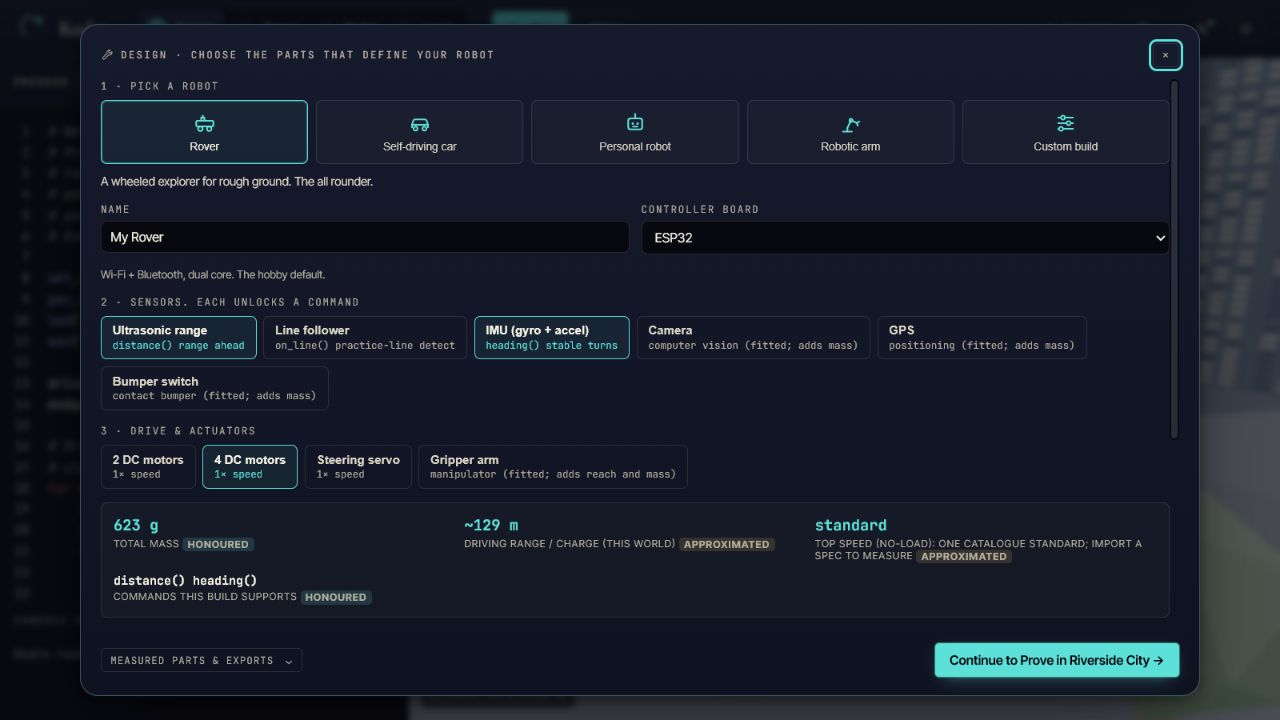
\includegraphics[width=0.56\linewidth]{img/simple_design.png}
\caption{The redesigned Robot Lab in the default Simple experience. Robot type, board, sensors and actuators remain available in one focused surface, while fidelity badges and the next Design-to-Prove action stay visible without exposing every instrument at once.}
\label{fig:lab}
\end{figure}

\section{A less-is-more interaction model}
The primary journey has three stages: Design, Prove and Build. Simple is the default for a first time or occasional user. Design contains the robot choices and a single next action. Prove opens a mission cockpit rather than the programming environment. It presents the robot, world and test as three plain choices, computes a deterministic readiness judgement before the run, and exposes one Run this test action rather than duplicating Run in the global toolbar. The same surface changes from preparation to live, paused and completed states, with distance, remaining battery and closest obstacle shown after an exact run. A stored result is displayed only when its robot, world and source program match the current plan, which prevents stale evidence from being mistaken for the latest test. Build turns the active design and evidence into an explicitly provisional build brief. Editing is a deliberate transition through Edit program, and the local Companion remains visible as the route to assisted construction. Lessons, teacher progress, replay, blocks, simulation limits and project history sit behind one More Tools control instead of competing with the primary stages. Expert is an explicit setting that restores the persistent editor, console, evidence rail and denser controls for a user who needs them. The selected level is stored locally. Nothing is removed from the underlying product, so an expert does not lose capability and a beginner is not forced to understand every panel before the first run. At mobile widths the same three stages become a fixed bottom navigation, and the secondary tools remain available through the same More Tools route.

\subsection{Input, process and output by stage}
The three-stage shell is an input-process-output model made visible to the user. Table~\ref{tab:ipo} records the contract of each stage and prevents a presentation-only redesign from obscuring what the system actually does.

\begin{table}[h]
\centering\footnotesize
\renewcommand{\arraystretch}{1.1}
\begin{tabular}{p{1.7cm}p{3.9cm}p{4.2cm}p{3.8cm}}
\toprule
Stage & Input & Process & Output \\
\midrule
Design & Catalogue choices or an imported measured specification & Derive mass, motion values, fitted capabilities and fidelity tiers & Active robot specification, command set and disclosed assumptions \\
Prove & Active build, program, world, contract and seed & Validate commands, run the deterministic engine and score immutable criteria & Seeded manifest, PASS or FAIL verdict, metrics and simulation-boundary report \\
Build & Active specification and the latest matching evidence & Summarise requirements and distinguish honoured, approximated and unverified values & Provisional build brief for competent datasheet and safety review \\
\bottomrule
\end{tabular}
\caption{The input, process and output contract of the three primary stages.}
\label{tab:ipo}
\end{table}

\section{The robot specification as the single source of truth}
The most important design decision in Kodro is that the robot is not cosmetic. Its specification is a single object that the rest of the system reads, and it is the reason changing the build changes the behaviour. The specification arrives one of two ways. A non-expert assembles it in the Robot Lab, where a derive step computes from the chosen parts a structured build: the chassis type, the board, the fitted sensors and actuators, and from those a mass in kilograms, a top speed, an acceleration, a turn rate, a battery capacity and a drain rate, a friction profile, and crucially a list of supported commands. A builder with a real machine instead imports a Kodro Robot Specification, a small JSON document validated by a schema in \texttt{specschema.js}. It carries the total mass, the body footprint in centimetres, the drive geometry (wheel radius, wheelbase, motor count and per-motor no-load rpm, stall torque and nominal voltage), the battery capacity, voltage and usable fraction, and the sensors with their mount position, yaw and range. The schema drops unknown keys with a warning, clamps mildly out-of-range values visibly rather than silently, and rejects wild ones, and it round-trips: a build can be exported back out as a specification for a peer to import. From that point the imported numbers, not a catalogue proxy, drive the simulation.

The command list is what makes the design honest. The registry is generated from the specification rather than written independently per panel. A build without an ultrasonic sensor has no distance-reading command in the registry, so the editor rejects it and the blocks palette does not offer it. The model is told the same registry, but may still emit an unavailable call. Validation then withholds that output. This distinction between reducing an error through grounding and enforcing the boundary through deterministic rejection is central to the safety claim.

The physical fields drive the motion. For an imported build the top speed follows a closed form from the motor rpm and wheel radius, the tractive force from the stall torque and motor count, the acceleration and braking from that force against the mass, and the battery runtime from the capacity against the drawn power. For a catalogue build the same character is derived from the chosen parts. Either way a heavier robot has a lower acceleration and a faster battery drain, a stronger motor raises the top speed, and the surface traction changes how the robot holds the ground. The point is that these are not separate sliders the user tunes. They fall out of the specification, so the design loop is to change the robot, not to change a number, and to watch the behaviour change as a consequence.

\section{The three-tier fidelity disclosure}
A proving ground earns trust by being candid about its own limits, so the second load-bearing design decision is that every figure the simulation reports carries a disclosed level of fidelity. Three tiers do the work. A figure is \textbf{honoured} when the simulation actually runs the measured number: the commanded distances and turn angles, the collision circle sized from the body footprint, the command availability gated on fitted parts, the battery treated as a hard budget the robot halts at, and, when a build's motor-derived top speed falls inside the simulable band, that top speed itself. A figure is \textbf{approximated} when a first-order model stands in for the real physics: acceleration and braking as a trapezoid rather than an integration of forces, turn timing from track geometry rather than wheel torque curves, traction as three coarse bands per surface, and battery drain as a constant-power ledger with no voltage sag or thermal derating. A figure is \textbf{not simulated} when it is reported for reference but never actually driven: slopes and terrain height, wheel-level slip and per-motor torque curves, suspension and three-dimensional contact, the water, depth pressure and vacuum of the underwater and space sites (which change gravity, traction and light only, so a clean run there is scoped to the surface and never claims the build would survive the hazard itself), and the command semantics of the parts that carry no runnable command yet.

The discipline of this scheme is that it is enforced at the edges, not asserted in prose. A top speed that falls outside the band the simulation can run is a case worth dwelling on, because it is exactly where an honest tool is tempted to cheat. A cheap educational rover with a slow motor has a real top speed below the simulable floor. Rather than run it at its true crawl, the simulation runs it at the floor, which is faster than real. The honest response, and the one the code takes, is to refuse to badge that number honoured: the badge drops to approximated and the warning states the real direction, that the top speed is below the floor and is simulated faster, rather than papering over the substitution. The same holds at the ceiling for a fast build. This case matters because it is the precise failure the whole product exists to prevent, a distorted number shown under a reassuring badge, and the design closes it by making the badge follow the truth of what the simulation runs. The tiers are surfaced three ways: as per-figure badges beside the live specification in the Lab, as a full table in a realism dashboard, and as a per-robot verification report, a standalone document that lays out the build as simulated with each figure tagged by tier and by how it was derived, for a skeptical builder to keep and check.

\section{One shared motion model}
\label{sec:shared-motion}
The third design decision answers a question the first two raise. If the imported specification drives the simulation, and the fidelity badges promise that a figure is honoured, then the number the user sees in the visible studio and the number a test asserts in the Python engine must be the same number, or the honesty is a fiction. Early in the project they were not the same. Four hand-rolled kinematic replicas, one in the JavaScript studio, one in the Python engine, one in the scenario validator and one in the self-test, drifted apart until they disagreed by an order of magnitude on how much battery a metre of travel costs. The design response was to collapse them into one shared motion model: a single set of closed-form equations and named constants, expressed once and mirrored in two files, \texttt{motion-model.js} for the studio and \texttt{engine/motion\_model.py} for the Python engine.

The model is locked at three levels, each a gate in continuous integration. The constant table is hash-gated: both files serialise their constants to a canonical form and a test fails if the two hashes differ, so a constant cannot be changed in one engine without the other. The catalogue-mode behaviour is golden-trace-gated: a corpus of programs is run through both engines and their displacement, distance, heading and battery are asserted to agree, so a change that alters how a robot moves fails unless both engines change together. Most recently, the physical-mode closed forms are formula-parity-gated: the fourteen closed forms plus the sensor-pose transform were ported from the studio's JavaScript into the Python engine, and a test runs the studio model over a reference robot and fails on any drift. An imported build's derived numbers, its top speed, stall force, mobility, acceleration, energy, runtime, slope, turn timing, stopping distance and sensor pose, are therefore provably identical across the two engines. The honest scope of this parity is stated plainly in the limitations chapter: the two engines share the formulas, but the full end-to-end simulation of an imported build, in particular the sensor rays that account for a sensor's mount pose and range, runs only in the studio, while the Python engine reproduces the derived numbers and grades catalogue-mode motion. The design goal was never to claim identical simulators. It was to make the numbers the fidelity badges rest on impossible to fake in one engine and not the other.

\section{The trace-driven core}
A single abstraction underpins scoring, hinting and replay: the trace. Every call the running program makes to the command surface appends an event that records the call, its arguments, its result, a snapshot of the robot's state, and any collision. From this one trace three features are derived without duplicating the representation of what the robot did. Scoring compares aggregates of the trace, the samples collected, the collisions, the battery used, the distance, the final position, against the scenario's declared success criteria, and an analysis of the source against the allowed constructs, to yield a pass or fail, a score, and a per-criterion reason. Hinting runs a set of rule predicates over the same events plus the score and surfaces the first that matches. Replay reconstructs the run from the serialised trace and scrubs through it.

The value of this choice is that the decision logic is pure. The scorer is a function from a scenario, a trace and the source to a result, with no input or output and no hidden state, which makes it trivially testable with synthetic traces and impossible to make non-deterministic by accident. The same purity holds for the hint rules and the report. Side-effecting wrappers, the file writes and the dialogs, are thin shells over these pure cores. This is why the system can be tested thoroughly without a display, which the evaluation chapter relies on.

\section{Safety: the sandbox, the executor, and the gate}
The user's program is untrusted, and the design treats it that way at three points. Before execution, the sandbox walks the program's syntax tree and rejects unsafe imports and builtins, the file opens, the process spawns, the attribute walks that reach for forbidden capabilities. During execution, the executor runs the program in a daemon thread under a hard wall-clock timeout, folding every failure mode, a syntax error, a runtime error, a sandbox violation, a timeout, into one structured result rather than letting an exception escape. After execution, the simulation gate is the run itself: the program drives the robot in a world and is scored, so a wrong program fails visibly on screen against the scenario rather than silently on real hardware.

These three points are the concrete form of the central analysis from Chapter~3. The model never touches any of them. It cannot relax the sandbox, it cannot extend the timeout, and it cannot decide that a program passed. The deterministic layer owns safety end to end, which is what lets the model be helpful without being dangerous.

\section{Worlds, mission sites, and moving agents}
The validation has to happen somewhere believable, so the design recommends a world to fit the robot. A self-driving car is dropped into the City, with one-way lane traffic that loops and brakes for the robot and pedestrians that keep to the pavements and use the crossing. A home or arm robot is dropped into the Room, with furniture and people. A rover is dropped onto a planetary terrain. Beyond these base worlds sit seventeen named mission sites, real places given their own treatment: the Sahara, the Amazon, Antarctica, the Thar Desert in India, the Maasai Mara, the slopes of Mount Fuji, the Giza plateau, an Icelandic lava field, the Himalayan foothills, the Great Barrier Reef, the Mariana Trench, Olympus Mons on Mars, the Moon's Tycho crater, Europa's ice crust, a robotics test bay, a warehouse and a minimal debug grid. Each carries its own traction, lighting and atmosphere, so the same program behaves differently across them and a run reads as a place rather than a plane. The open worlds are alive: traffic keeps to one-way lanes and eases rather than stepping, pedestrians walk their pavements and a few cross at the crossing, and a small autonomous fleet of other robots roams the open terrains, picking fresh goals and steering around the obstacles, each other and the user's robot, so the scene has machines to share it with rather than being an empty stage. Figure~\ref{fig:city} shows the City world in three dimensions, which the user can orbit a full turn to read the scene from any angle.

\begin{figure}[t]
\centering
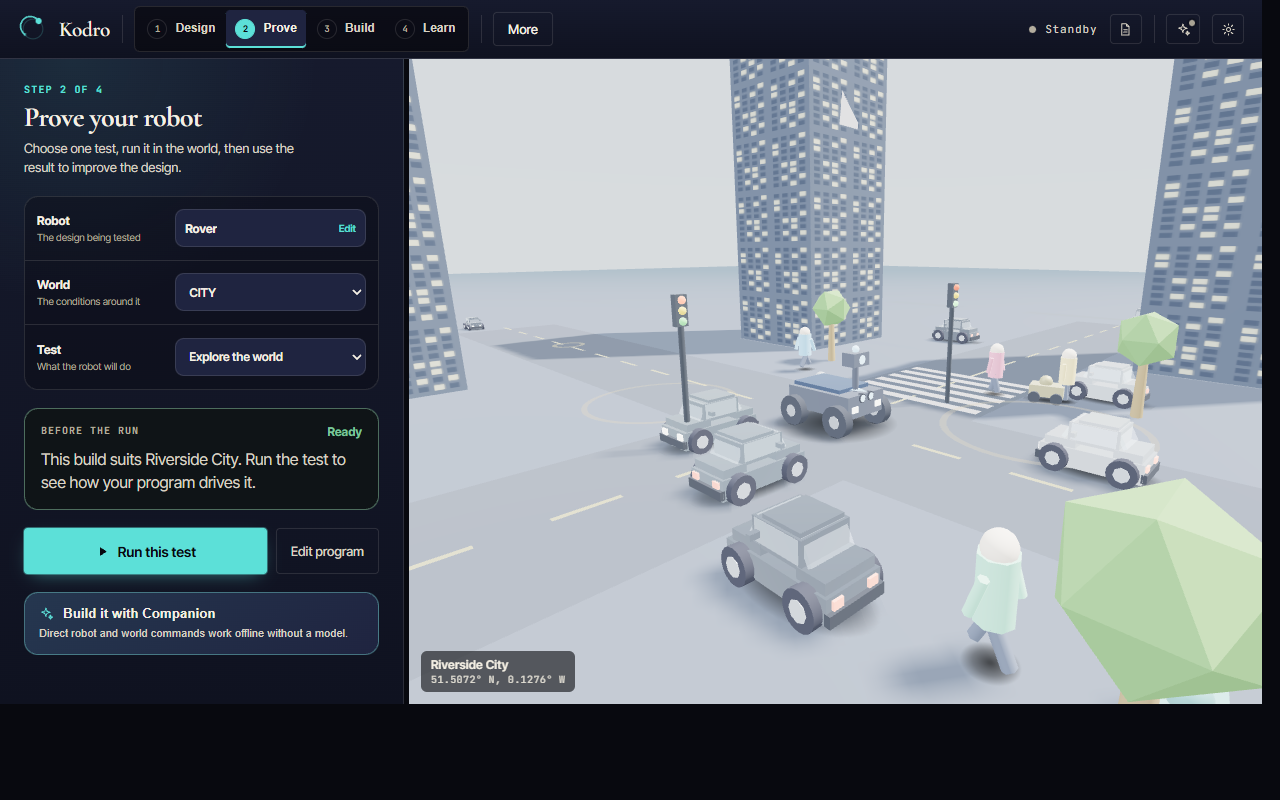
\includegraphics[width=0.56\linewidth]{img/simple_studio.png}
\caption{The default Simple proving surface. The mission cockpit exposes only the robot, world, test, deterministic readiness check and one Run this test action beside the three dimensional City. Program editing and the evidence history are deliberate transitions rather than permanent panels.}
\label{fig:city}
\end{figure}

The motion is designed to read as natural rather than to be physically exact. The robot does not slide like a prop. It transfers weight under acceleration, banks into turns, settles on its suspension, and steers from the front wheels where the chassis has them. The honest description of this, returned to in Chapter~7, is that it is a per-type kinematic model that fakes the feel convincingly rather than a rigid-body solver that resolves forces. This is a deliberate trade. The believable feel is what a non-expert needs to judge a behaviour, and it runs smoothly on a laptop, where a full solver would not.

\section{The grounded assistant and its deterministic fallback}
The assistant is designed around the principle that the model may generate but validators decide. It receives the robot specification and command registry, which is the fixed-interface form of grounding that follows from asking a model to compose a known capability set rather than to invent one \citep{liang2023,ahn2022}, then normalises known compatibility call styles and validates the resulting syntax tree against that set \citep{khati2026}. When a request needs a part the build lacks, Kodro returns the missing-capability error and exposes no Apply action. Bounded repair is allowed, but a failed repair remains a refusal rather than a plausible program. The automatic reviewer follows the same rule: a proposed rewrite is accepted only after validation, otherwise the original is retained with the rejection reason.

Behind all of this is the deterministic fallback, which is what makes the offline guarantee real. If no model is installed, or if the model does not answer within a fixed time budget, a rule engine returns rule-based code and checks, and the platform stays fully usable. The fallback is not a degraded mode bolted on. It is the floor the whole assistant stands on, and the design treats the model as an optional accelerator above a guaranteed deterministic base.

\section{Self-refinement without retraining}
The final design element is a memory loop. Three local, countable mechanisms carry it. After a run the system stores a reflection and can retrieve related notes for a later suggestion. Validated routines can be saved as named skills, and past designs remain available for inspection. None of this edits model weights. It is system-level retrieval, and calling it an improvement would require the planned controlled ablation. The present evaluation demonstrates storage, retrieval and display, not a fall in iterations.

\section{The lesson path and its single source of truth}
\label{sec:lesson-design}
The teaching half of the product is the largest part of it, and it is designed around one constraint: a lesson must not be able to say one thing on screen and be marked as another. The constraint is met by giving each lesson exactly one definition and deriving every other view of it from that definition.

A lesson is therefore a validated document rather than code. Each bundled lesson is a schema-checked file carrying its key stage, its computational-thinking concepts, its curriculum references, the world the learner will see, the starter program, the constructs the learner is permitted to use, a line budget, a hint bank, an optional reading age and glossary, one worked answer, and its success criteria. A criterion is drawn from a closed set of eight machine-checkable properties: samples collected, a battery ceiling, absence of collision, use of a named construct, return to base, a step ceiling, a distance floor, and an ordered list of calls that must occur. The set is closed on purpose. A criterion that cannot be expressed within it cannot be written, so every lesson's definition of done is executable rather than editorial, and the marker can never be asked to judge something it has no way to measure. The ordered-calls property is the clearest illustration of why the set grew rather than being designed once: it exists because a lesson that told the learner to call three functions in order previously passed a program with two of them deleted.

Two marking engines consume that one document. The desktop build marks in Python; the browser build marks in JavaScript against a compiled copy of the same library exported into the web assets. Neither engine owns a lesson's meaning, and a disagreement between them is a gate failure rather than a matter of judgement. This mirrors the arrangement already described for the motion model in Section~\ref{sec:shared-motion}, and it is the same argument: two independently written implementations of one specification are only safe if their agreement is enforced by a machine.

The marking target is the run the learner watched. The lesson's world is the world rendered on screen, the sensors read that world, and the mark is computed from the trace it produced. This sounds obvious and was not the original behaviour: an earlier design held the lesson's obstacles and samples inside the marker alone, so a learner could watch the robot strike a rock and then be told there were no collisions. Where the desktop build re-executes the program to mark it, because the learner record and the adaptive hints live on that side, the second run is disclosed on screen rather than unified away at the risk of breaking the record.

Help is ordered, and authoring uses the same path as consumption. A learner who stalls receives the lesson's hints in sequence, and the worked answer is withheld until they are exhausted; the worked answer exists both so that a stuck learner has a floor and so that solvability can be gated, which Section~\ref{sec:classroom-gates} describes. A lesson written in the Lesson Studio produces the same document, is checked by the same validator, and cannot be saved until the author's own answer passes the marker the learner will face, after which it is graded by identical code to the bundled library and exports as a single file. The learner record itself is deliberately unremarkable: names, programs and attainment are written to local storage on the machine, are readable and deletable by the operator, and are never transmitted. The design consequence of that choice, and the obligation it places on a classroom operator, is taken up in Chapter~8.

\chapter{Implementation}

This chapter describes how the design was realised. It is grounded in the codebase and in the running test-evidence log, and the engineering challenges are drawn from the real commit history, which makes them honest material for critical reflection rather than a tidy story told after the fact.

\section{The program surface and the interpreter}
The user's program runs through a Python subset interpreter, written in JavaScript and vendored into the bundle, which compiles a source string into a generator that yields motion and sensor events one at a time. The generator design is what lets the studio animate a run smoothly: the application pumps the generator, advancing the robot one event per tick, so the user sees the robot move rather than jumping to a final state. The interpreter supports the constructs a non-expert needs, sequence, selection, iteration with both \texttt{for} and \texttt{while}, functions, and the sensor reads, and it guards the pathological cases a beginner can stumble into, such as an enormous exponent, so that a slip produces a contained result rather than a hang.

A subtlety worth recording is that two call styles are both valid and both correct. A bare call such as \texttt{move\_forward(2)} moves two metres, scaled internally to engine units, while a method call such as \texttt{rover.forward(200)} moves two hundred centimetres. This dual surface is convenient but it is also a known source of the arena-scale mismatch discussed in Chapter~7, and it is recorded honestly rather than hidden.

\section{The robot specification and the derive step}
The Robot Lab implements the single source of truth from the design. A catalogue of boards, sensors, actuators and chassis types backs a derive step that computes the structured specification from the chosen parts. The derive step is where the physical character of the robot is set: the mass is summed from the parts, the top speed and acceleration follow from the motor and the mass, the battery capacity and drain follow from the board and the load, and the supported-commands list is assembled from exactly the parts that provide each command. Saving a build dispatches an event carrying the recommended world, which the studio listens for, so designing a robot and being dropped into the right world to test it are one action.

\section{Importing a real robot: the KRS schema}
Alongside the catalogue sits the import path, which is what makes Kodro a proving ground rather than only a studio. The Kodro Robot Specification is a JSON document with a schema and a validator in \texttt{specschema.js}. A builder presses Import spec, the desktop bridge or a file dialog reads the document, and the validator returns a cleaned specification with a list of warnings and errors surfaced in the Lab. The validation is deliberately forgiving where it can be and strict where it must be: an unknown key is dropped with a warning rather than rejected, a value mildly outside its band is clamped and the clamp is shown, and a value wildly out of range is refused outright, so a hand-written or third-party specification imports usefully without silently becoming a different robot. When a specification carries motor and drive geometry, the physical closed forms take over from the catalogue proxies: the derived object carries a \texttt{phys} block whose numbers, not a parts factor, drive the simulation. The same schema exports, so a build assembled in the Lab or imported and adjusted can be written back out as a specification for a peer, and the export carries the derived numbers alongside the inputs so the receiving side can check them.

\section{The shared motion model and its conformance gates}
The one shared motion model of the design is two mirrored files. \texttt{motion-model.js} holds the constants and the closed forms for the studio. \texttt{engine/motion\_model.py} holds the twin for the Python engine. The physical closed forms are the load-bearing part: the top speed as $v = (\mathrm{rpm}/60)\,2\pi r$, the tractive force as motor count times stall torque over wheel radius, the acceleration as that force less rolling resistance over mass, the battery drain from a rolling-resistance power model against the usable energy, the differential turn timing from track geometry and the Ackermann turn radius from wheelbase and steering angle, the stopping distance as $v^2/(2\mu g)$, and the sensor-mount transform that places a sensor's reading at its offset and yaw.

Three tests gate the pair on every push. A conformance test serialises both constant tables to a canonical form and compares their SHA-256 hashes, so a constant edited in one engine and not the other fails the build. A golden-trace test runs a corpus of programs through both engines and asserts their displacement, distance, heading and battery agree, so catalogue-mode motion cannot drift. A physical-golden-trace test runs the studio's closed forms over a reference robot through a small Node fixture and asserts the Python twin returns the same values to within a relative tolerance of \(10^{-12}\) or an absolute tolerance of \(10^{-9}\), whichever is the looser bound at that magnitude, so the derived numbers an imported build shows are the same on both sides to far below any figure the interface displays. The absolute bound is the binding one for every quantity smaller than \(10^{3}\), which is most of the trace, and it is stated here rather than quoting the relative figure alone.

The honest boundary, recorded in the limitations chapter, is that the Python engine's sensor rays still originate at the rover centre with fixed module ranges and do not yet consume an imported sensor's mount pose or range, and the public Python API does not import a specification's mass, rpm or battery, so a measured build is simulated end to end only in the studio while the Python engine mirrors the formulas and grades catalogue-mode motion.

\section{The verification report}
The fidelity disclosure is implemented as pure functions in \texttt{verify.jsx} that turn the active build into a prediction sheet and join it with the evidence the app already holds, the last live run's odometer and wall-clock and the last multi-seed validation report. Every row carries its figure, its value, its fidelity tier and a one-line statement of how it was derived, for example that a top speed came from $v = (\mathrm{rpm}/60)\,2\pi r$ on the imported motor rather than from a catalogue anchor. The report renders to a standalone HTML file a builder can save and keep, and because the functions are plain JavaScript with no React they are exercised headless by the QA harness. Nothing in the report computes new simulation state. Every number is either a motion-model closed form or a recorded result, which is what lets the report make its honesty claim truthfully.

\section{The worlds and the natural-motion tick}
The three-dimensional 3D Viewport is built on core Three.js with no asset loader, so every robot, obstacle, terrain feature and agent is procedural geometry generated in code, boxes, cylinders, spheres, extruded shapes and canvas textures, lit by an environment map with shadow mapping and tone mapping. The open-terrain ground is shaded rather than flat: a tileable normal map, derived by a Sobel pass over a periodic height field, and a roughness map are both generated in canvas at scene-build time, so the sun and fill light graze real micro-relief instead of a coloured plane. The City and the Room are built in code, and the moving agents, the traffic and the pedestrians, run in a shared coordinate space with one-way lanes, looping paths, and a rule that brakes them for the robot. The natural-motion tick is the code that gives each robot type its feel: the per-type pitch under acceleration, the roll into a turn, the suspension settle, and the front-wheel steer, applied as a function of the robot's velocity and heading change each frame. The world is chosen from a catalogue of presets, the City and the Room alongside a Robotics Lab, a Warehouse, a Minimal Debug Grid and a set of real outdoor terrains, each carrying its own friction and lighting so the same program behaves differently across them.

A render-quality control spanning Low to Cinematic bounds the two heaviest costs, the shadow resolution and the pixel ratio, so the scene stays smooth on a laptop with no discrete graphics card on the lower tiers and maxes its fidelity for a screenshot on the highest. The Cinematic tier additionally runs a small, hand-written, fully offline post chain, a bloom built from a bright-pass and a separable Gaussian blur composited additively over the base render together with a vignette, written directly against the core renderer because the library ships its post-processing only in an examples tree that is not vendored and cannot be fetched under the offline rule. The pass is gated so that it is disabled under a reduced-motion preference, turned off if the slow-hardware downgrade fires, and dropped to the plain render if the device cannot allocate its targets, so the offline and low-hardware guarantees hold on every tier. A first-person toggle drops the camera onto the robot for a driver view.

\section{Offline shading without an asset pipeline}
The offline rule shapes the renderer as sharply as it shapes the model. The single largest lever for visual quality in a real-time scene is usually an asset pipeline: a glTF or GLB loader and a set of authored, well shaded models. That lever is closed here. Three.js ships its loaders and its post-processing only in an examples tree that is not part of the vendored core, and the zero-network constraint means neither the loader nor any quality interchange model can be fetched and committed. A hand-authored model would in any case be no better than the procedural geometry it would replace. The honest design response is to push the procedural surfaces as far as they will go and to be candid that an importer is future work rather than a missing feature that was skipped.

Two pieces of that work are worth recording because they were done under the constraint rather than around it. The first is surface relief. The open-terrain ground already carried a baked colour grain, but light still struck it as if it were glass, which was the strongest tell that the world was a tech demo. Each ground now generates, in canvas at scene-build time, a tileable normal map together with a roughness map. The normal map is a Sobel pass over a periodic height field whose waves are integer multiples of the tile size, so the derived normals are seamless under repeat wrapping. The result is that the existing physically based sun and fill light graze real micro-relief, and sand reads as sand, regolith as pits, the seabed as ripples. No texture file is loaded and no new binary is vendored.

The second is a post-processing pass for the highest quality tier. Because the library's bloom pass is not available offline, the pass is written directly against the core renderer: the proven base image is drawn to the canvas exactly as the lower tiers draw it, the scene is then rendered once more into an offscreen target used only as a bloom source, and a bright-pass, a separable Gaussian blur, an additive bloom composite and a vignette are layered on top. Drawing the bloom additively over the unchanged base, rather than replacing the image, means the worst case is that the scene simply looks like the normal render, which makes the feature safe to ship. It is gated to the Cinematic tier, disabled under a reduced-motion preference, turned off automatically if the slow-hardware downgrade fires, and dropped to the plain render if the device cannot allocate its render targets or if the pass throws at frame time. The shading and the post pass are headless safe: with no document or WebGL context the generators return nothing and the scene renders exactly as before, so the offline bundle-render test never touches a canvas. This is the offline constraint treated as a design input, not an apology.

\section{Memory, the assistant, and the fallback}
The memory store records reflections and saved skills and retrieves them before selected suggestions, which is the verbal-reflection and reusable-library pattern identified in Chapter~2 \citep{shinn2023,wang2023} implemented as files on disk rather than as any change to the model's weights. The assistant can call a local Ollama server, lists the installed models and lets the user override the automatic model choice. It passes the active command set through both generation and review, normalises supported call styles, validates the syntax tree and fails closed after bounded repair. The same contract is implemented in the static browser build, where a hosted page may contact the user's loopback Ollama server only when that server permits the page origin. The deterministic rule engine remains the guaranteed path when a model is missing or unavailable. An explicit bring-your-own-key provider is also available. That connected mode transmits prompts to the selected provider and is outside the offline guarantee.

\section{Engineering discipline}
Each unit of work closed only when a full gate passed: the test suite with branch coverage, the linter, the format check and a strict type check, after which the change was committed, pushed, and verified green on continuous integration. The coverage gate ratcheted upward as the codebase matured and settled at a minimum of eighty five percent line and branch, which every push must clear to merge. This discipline is itself a contribution, because the decision log and the test-evidence log it produced give the claims in this dissertation an audit trail that can be checked against the repository.

\section{Representative listing}
The scorer illustrates the trace-driven, pure-core principle from the design. It takes a scenario, a trace and the source, and returns a structured result with no input, no output and no hidden state, which is exactly what makes it testable with synthetic traces.

\begin{lstlisting}
@dataclass(frozen=True, slots=True)
class GradeResult:
    passed: bool
    reasons: list[str]   # one user-facing line per failed criterion
    score: int           # 0 to 100

def grade(lesson: Lesson, tracer: Tracer, source: str = "") -> GradeResult:
    aggregates = _compute_aggregates(tracer.events())
    reasons: list[str] = []
    for criterion in lesson.success_criteria:
        reason = _check_criterion(criterion, aggregates, lesson, source)
        if reason is not None:
            reasons.append(reason)
    score = max(0, 100 - SCORE_PENALTY_PER_FAILURE * len(reasons))
    return GradeResult(passed=not reasons, reasons=reasons, score=score)
\end{lstlisting}

\section{Showcases, icons, and project files}
Three showcase programs ship as example tabs and double as living documentation of the command surface, each verified to run in the interpreter QA sweep. Encore is the flagship: functions, loops, nested loops, counters and pen geometry over the base command set alone, so it runs on every build and shows the language working. Searchlight is a battery-managed survey and rescue mission, a robot given real work, running a systems check and patrolling a search area with every drive guarded by the distance sensor so it never touches a wall. Gauntlet is a capability reference that draws its own proof, exercising recursion, nested loops, chained comparisons, list building and a run of pen geometry. Around these, the interface chrome was professionalised: a procedural SVG icon set replaces every emoji-as-icon, each icon a handful of primitives built offline against \texttt{currentColor} so it renders identically on every operating system, which the interpreter QA enforces by asserting zero emoji glyphs remain in the chrome source. A whole project, the build, the programs, the active world, the render settings and the accumulated memory, serialises to and from a single \texttt{.kodro} JSON file with bounded sizes and a validator that never throws, so a session is portable and a backup is a file copy.

\section{The voice route, removed and rebuilt}
An earlier build offered a third way to program, a voice route with speech-to-text and a spoken assistant, and it was removed in full. The reason was a scope judgement made honestly: under the offline constraint the path could not be made reliable and cross-platform without depending on an optional component the design did not want to require, so rather than ship something fragile it was cut.

It was later rebuilt, and the earlier removal is what shaped the rebuild. The first attempt had treated speech as a third authoring route, which is precisely what made it fragile, because a mis-heard word became a wrong program with no obvious place for the pupil to notice the substitution. The rebuilt layer authors nothing. It speaks replies, and it dictates into the chat box that already exists, and every transcript is handed to the same parser that interprets typed text, so a spoken sentence reaches no action a typed one could not and skips no confirmation the typed path would have asked for. This is asserted as a property rather than assumed, by parsing a set of spoken phrasings and their typed equivalents and requiring the results to be identical.

The privacy position is split, and it is set out plainly here because it is the one boundary on the offline claim. Speaking is local: the layer accepts only voices the browser reports with \texttt{localService} set true, and on a machine with no local voice installed it turns speaking off and says why rather than falling back, because the network voices a browser lists in that same collection are served by sending the text away to be spoken. Listening is not local and cannot be made local in the browsers this targets, since the recognition interface delegates the captured audio to a vendor service. Which vendor is not the product's to know. The desktop build renders inside the platform web view rather than inside Chrome, so the recogniser it is handed belongs to whoever wrote that engine, and an earlier version of the opt-in that named one company was wrong everywhere that company's engine was not the one running. The wording now states what holds on every engine, which is that the recording leaves the machine, that the service receiving it belongs to the browser's maker rather than to the platform, and that the platform can neither choose it nor observe it. Naming a specific wrong recipient is a worse failure of consent than naming none, and the gate now forbids the notice from naming a single vendor at all. Dictation is off by default and reachable only through that opt-in before anything is enabled, it is withdrawable, and the microphone is never left open because recognition is requested one utterance at a time. A pupil who never turns it on sends nothing, and a school that forbids it can leave it off with no other part of the platform degrading. The visual \texttt{say} command is unrelated to any of this and remains what it always was, a console line the robot writes.

One hundred and eight assertions hold the layer, run in Node against its pure functions with no browser present: that a voice list containing only network voices yields no voice at all, that the opt-in notice says the recording leaves the machine and names no single vendor as its destination, that dictation is off until consent is given and goes off again when it is withdrawn, that spoken sentences parse identically to typed ones, and that the spoken form of a reply never reads a code block aloud. Eighteen of those assertions pin the verbatim output of a local recogniser rather than a guess at it, and they exist because a measured benchmark contradicted the code. A small offline transcriber was run over ten synthesised clips of the product's own five commands, recorded in \texttt{docs/eval/stt\_bench.json}; it never once returned the product name as spelt, producing \emph{Caudreau}, \emph{Cottro} and \emph{Caudrill} instead, none of which the shipped list of expected mishearings held. The consequence was not cosmetic. With the name left in front of the sentence, \emph{how do I make the rover go faster} parsed as a command and set the speed, and every spoken \emph{stop} failed to interrupt a reply. The rule was replaced by a phonetic test on the leading token and the ten transcripts are now pinned in the gate, along with the words the rule must not consume, \emph{quiet} first among them because it is itself an interruption.

Fourteen of those assertions cover the thing the layer has to reach if it is to be more than a novelty, which is the lesson library. A lesson resolves whether it is named by topic, by title or by number, and the ordering of the routing table is asserted so that a specific lesson wins over the generic one whose own title contains the same word. The near-misses are held as tightly as the hits, because opening a lesson resets the stage and swaps the program buffer, so a question about a lesson, a hypothetical about starting one and a request to write code for one all leave the library where it was. That routing table is a second copy of a fact the library already owns, so it is gated in both directions: a test fails if the table names a lesson that is not shipped, and fails again if a shipped lesson has no phrase that reaches it, which is what stops a new lesson from being reachable by mouse alone.

\section{Two front-ends over one engine}
The interface exists in two forms over the same engine. The original is a Tkinter interface that ships with Python and renders on any machine, retained as the guaranteed-offline fallback. After formative review found the Tkinter look dated for an audience that benchmarks software against web and mobile apps, a second front-end was added in the medium the reference design was authored in, a vendored offline React interface rendered in a pywebview window. Both front-ends drive the same engine, scorer, library and store. The honest risk here, recorded in the next chapter, is the dual interpreter: the web interface ships its own JavaScript interpreter for instant animation, whose surface differs from the Python API, and the planned convergence is to stream real engine events to the view and retire the second interpreter.

\section{A third surface, for programs rather than people}
The two front-ends are both for people. A third surface exists for software, exposing the same engine to an external agent over the Model Context Protocol. It offers eight tools, which list the lesson library and fetch a single lesson, run a program and grade one against a lesson, check a call against the robot command surface, validate a robot specification, prove the motion contracts, and report a pupil's progress. Alongside them sit twenty-five readable resources, the command reference and one per lesson in the library.

Two properties of that surface matter more than its contents. The first is that it answers out of the same engine, grader and library the pupil's own interface uses, so an agent cannot obtain a verdict the pupil could not obtain, and a lesson cannot be marked passed by a route that skips the sandbox. The second concerns the offline claim. The protocol layer is written directly against the Python standard library, speaking JSON-RPC over standard input and output, rather than by installing a protocol package. That is a deliberate cost: a hand-written transport is more code to be responsible for than a dependency would have been. It is paid because the alternative would have made the central claim conditional, since a platform that requires a package index before it can be integrated is no longer a platform that runs on a school machine with no account and no network. The server opens no socket and makes no request of its own. What chooses to connect to it, and whether that client is itself local, is the operator's decision and is outside the boundary this dissertation claims for the platform.

\section{Challenges met and fixed}
These are real defects, found and fixed, and they make the strongest reflection points.

\begin{itemize}
\item \textbf{A procedural surface over a stateful engine.} A flat set of free functions has to reach a single live engine. This was solved with a module-level binding that the functions consult at call time, which also let the headless tests and the scorer drive the engine with no interface present.
\item \textbf{An open loop.} An early build ran the user's program but never responded to it, with no pass or fail and no feedback. The fix wired scoring, hinting, persistence and the verdict into a single finish step at the end of every run, which a structured review had identified as the single biggest weakness of that build.
\item \textbf{A silently detached trace.} While fixing the loop, the active trace could be detached between runs, so a run recorded zero events and some integration tests passed vacuously. The fix re-asserts the trace and engine bindings at the start of every world reset, and the tests were strengthened to prove real movement, since the battery only drains if the robot actually moved.
\item \textbf{Four kinematic replicas that had drifted.} The studio, the Python engine, the scenario validator and the self-test each carried their own copy of the motion arithmetic, and they had drifted until they disagreed by an order of magnitude on battery cost per metre. The fix collapsed them onto the one shared motion model and locked it with the constants-hash, golden-trace and formula-parity gates, so the number the fidelity badges rest on cannot differ between engines again.
\item \textbf{Two honesty defects in the fidelity surfaces.} A panel review of the version 2.0 build found the two most damaging kind of defect for a proving ground, a sim that tells the user a false thing about a real build. A slow imported robot was simulated faster than its real top speed while still badged honoured, with warning copy that named the wrong direction. The predictive design check used a different mobility model from the live simulation, so the two headline surfaces contradicted each other on the shipped reference robot. Both were fixed: the top-speed badge now drops to approximated and states the true direction when the speed falls outside the simulable band, and the design check drives its mobility verdict from the same force-ratio model the simulation uses when an imported build is present. These are recorded here rather than buried because they are the clearest evidence that the honesty discipline is enforced by review and repair, not merely asserted.
\item \textbf{Headless interface fragility.} A modal error dialog blocked forever on the headless test runners, once burning a job to the six-hour ceiling. A per-test timeout was added so any hang fails fast with a traceback, which then pinpointed further headless issues and led to treating one platform's interface tests as informational while the other two remain hard gates.
\end{itemize}

\section{Packaging}
The desktop binary is built with PyInstaller, which bundles the interpreter, the runtime, the libraries and the asset bundle into a single windowed application, so deployment is one download with no separate runtime install. The build is reproducible from a specification file and was smoke-tested on a real desktop, where the packaged application starts cleanly and renders the full interface, which the headless suite otherwise exercises without a display.

\section{Web deployment}
The desktop application remains the full-featured path, but the same vendored interface now also ships as a zero-install web build. A flag on the bundle build script emits a fully self-contained static site, plain files with no server-side component, which a continuous-integration workflow deploys to GitHub Pages, so the studio can be tried from a link without installing anything. The offline character survives the move in two ways. First, the build is a progressive web application: a manifest and a service worker precache the application shell, so after the first load the site keeps working with the network off. The service worker serves same-origin requests cache-first and never touches a cross-origin request, so a call to a user's own optional cloud key or to a localhost Ollama server can never be intercepted, cached or leaked by the caching layer. Second, the privacy claim is enforced by a gate rather than asserted: a dedicated check builds the static site, serves it from the loopback address, loads it in a headless browser under a network log, and fails if the default page makes a single request to any external host, alongside a proof that the application actually boots.

What runs where is stated precisely because the two builds have different persistence boundaries. The simulation core is client-side JavaScript in both: the interpreter, randomised validation, worlds, three-dimensional viewport, Robot Lab, verification report, memory and assistant provider layer. The lesson library is generated from the desktop source and parity checked. The browser now grades lesson attempts through a JavaScript grader, supplies progressive hints and stores a combined concept-strength record in that browser. The desktop bridge retains separate pupil identities and the fuller teacher record. Browser classroom evidence is therefore functional but not multi-pupil. Both modes use the same build-aware validation contract for model code.

\section{The lesson library, the two markers and the learner record}
The lesson path of Section~\ref{sec:lesson-design} is implemented as one authored source and two consumers. The library is a directory of schema-validated lesson files loaded and checked by a typed model, so a malformed lesson fails at load rather than at the moment a learner meets it; the schema forbids unknown fields, requires at least one concept and one permitted construct, and rejects a success criterion that sets none of its eight properties. An export step compiles the validated library into a single JSON document placed in the web assets, which is what the browser build reads, and a unit test fails whenever that document falls out of step with the source. The library is therefore authored once in a form a person can read and diff, and shipped in a form a browser can fetch, with the gap between the two closed by a test rather than by discipline.

Marking is implemented twice because the two builds have different jobs. The Python grader serves the desktop path, where the learner record and the adaptive hints live; a JavaScript grader in the bundle serves the browser path, where marking has to happen against the trace the learner just watched with no server to call. Both read the same criteria and both dispatch on the same closed property set, which is what makes the parity gate meaningful: the gate can only be written because there is nothing in one engine's notion of a pass that the other cannot express. Around the markers sit the smaller learner-facing modules, each with its own harness: a store that keeps names, programs and attainment in local storage, a class record and attainment roll-up for the teacher view, a reordering exercise type with its own distractor handling, learner-facing error text that maps every interpreter fault to a readable message, and the Lesson Studio, which reuses the validator and the marker so an authored lesson cannot be saved until the author's own answer passes.

The engineering difficulty here was not writing the markers. It was discovering, through two adversarial audits, that the learner was watching one simulation and being marked by another, and that several lessons could be passed without doing the thing they taught. Those findings, and the repairs that followed, are what the classroom gate set in Section~\ref{sec:classroom-gates} was built to prevent recurring.

\chapter{Evaluation}
\label{ch:evaluation}

This chapter records how Kodro was evaluated. It separates what was actually measured, the automated verification and an analyst-run formative review, from what is planned but not yet done, a study with real users. Nothing here reports data from human subjects, because that study has deliberately been left for a point at which it can be run properly under consent.

\section{Evaluation strategy}
Twelve methods were used, in increasing cost and decreasing frequency. Six are continuous automated gates that run on every push: the Python test suite, the interpreter QA harness, the world and interface nets, the Prove contract replay, the lesson solvability and marking gates, and the learner-record and error-path gates. Four are periodic measured studies: the formative persona review, the deterministic persona-task evaluation, the renderer evidence and the KodroBench grounding benchmark. One is the seven-round adversarial persona panel. The twelfth, a user and refinement study that would measure real efficacy and the effect of the refinement loop, is planned and has not been run, and no figure in this chapter comes from it. Table~\ref{tab:evalstrategy} in Appendix~\ref{app:evaldata} states what each method checks and its status. The sections below report each in turn.

\subsection*{Where the numbers in this chapter come from}
Almost every figure reported below is emitted by a harness into a versioned artefact under \texttt{docs/eval} rather than transcribed by hand; the two exceptions are named at the end of this paragraph. The Python matrix and its coverage are written to \texttt{test\_suite.json}, together with the commit and working-tree status of the run. The Prove contracts write \texttt{prove\_baseline.json} and the human-readable \texttt{prove\_report.md}, which carry the contract set, the engine, the seed root, the declared evidence boundary and the overall verdict. The renderer measurements are split across \texttt{performance\_eval.json} and \texttt{performance\_eval\_hardware.json}, one per graphics mode, each recording its method, the browser and platform it ran on, the 240\,Hz frame-time target it is judged against and hashes of the artefacts it measured. The interface gates write \texttt{ui\_eval.json} on the same pattern; a narrowed \texttt{--suite=} run writes its own per-suite file alongside it, and those partial files are deliberately kept out of version control so that a narrowed local run cannot be mistaken for the full one. The live-Ollama run writes \texttt{vibe\_eval.json} with its model, endpoint, per-measure results and totals; the synthetic-persona task evaluation writes \texttt{persona\_eval\_results.json} with its model, base seed, turn limit and cell count. Each of these files carries a schema version and a generation timestamp, so a reader can tell which run produced a number and whether the artefact matches the source state it claims. The first exception is the group of nine offline module gates reported later in this section, which print their totals to standard output and emit no JSON; their commands and printed lines are transcribed into \texttt{qa\_gate\_runs\_2026-08-14.md}, which says on its face that it is a hand-written transcript, so a reader checks those figures by re-running the command in its first column rather than by trusting the file. The second is the adversarial persona panel of Section~\ref{sec:panel}, whose round-by-round tallies were kept in session notes rather than emitted by a harness; that gap is stated again where the method is reported, because it is the one set of figures in this chapter a reader cannot re-run at all.

\section{Automated verification}
\label{sec:autoverify}
The primary evidence of correctness is the Python suite, which grew with the codebase and gated every change. At commit \texttt{e70b98b}, the complete declared matrix, including the optional RL and URDF surfaces, collects 1,641 tests at 90.85 percent branch-aware coverage against an 85 percent gate, and passes all of them. No test skipped in that run, and that is not the same as the host's intermittent Tk startup failure being fixed. The same matrix on this machine has reported one skip, then two, then none. Thirteen test files open a Tk window in a fixture that catches the startup error and degrades to a skip rather than a failure, and 169 collected tests sit behind those guards, so a clean run means the toolkit started on that occasion and nothing stronger. Because the cause is not established, the artefact records whatever skip its own run produced and attributes none. Those figures are not transcribed. They are generated from the run's own coverage report and JUnit output into \texttt{docs/eval/test\_suite.json}, which also records the commit and the working-tree status, so the count belongs to that commit and not to the \texttt{v2.0-submission} tag. The percentage is a floor rather than an exact figure, because the harness drops the coverage contribution of node-subprocess tests on this host while still running them and still counting them in the test total; continuous integration, which applies no such exclusion, measures the same suite at or above the quoted number. Unit, property-based and headless integration tests pin the procedural API, deterministic physics and scoring, sandbox rejection, hard timeout, shared-motion conformance and the run, score, hint and persistence loop. The separate interpreter harness passes 180 of 180 checks. Strict lint, format and type checks also pass, and the wheel builds successfully.

Alongside the Python suite, a separate interpreter QA harness drives the shipped interpreter with the real kinematics and the wall ray, and asserts the command semantics, every bundled example program including the three showcases, and a set of product-coherence checks. It passes at one hundred and eighty of one hundred and eighty. Every example terminates, moves, stays inside the arena, never hits a wall and never throws, and the command semantics, the two motion call styles, the turn, the speed clamp, the guarded huge exponent, the loops and the sensor reads, are each asserted, as are the interpreter diagnostics, the honesty of the design-check command list and the absence of emoji glyphs from the interface chrome. This harness is the evidence that the user-facing program surface behaves, independently of the Python engine.

The deterministic Prove gate covers four declarative contracts: straight transit, a corner route, obstacle clearance and battery reserve. Each contract is replayed over five seeds while obstacle offset, range noise, start delay and initial battery vary within declared bounds. The resulting manifest records the source SHA-256, contract identifier, seed, engine identity and source hash, sampled conditions, metrics and verdict. It deliberately has no wall-clock timestamp, so an identical source, contract and seed produce byte-identical JSON. The candidate baseline passes all twenty runs. A second replay is byte-identical, baseline comparison reports no regression, and an intentionally broken controller returns a failing process status with all four contracts failed. The human-readable companion report states that the evidence comes from a kinematic simulation and cannot certify a physical robot. The local Companion may interpret these records, but the verdict is calculated and owned by the deterministic runner.

Browser evidence is split so that a degraded launcher cannot be mistaken for a product result. The shipped static build passes five of five boot, mount and zero external request checks, and the deterministic stylesheet gate passes 74 contrast and responsive assertions over ten themes. The split headless matrix passes six of six rendered flows, 41 of 41 behaviour assertions, six of six layouts and 13 of 13 modal surfaces. Those checks cover program execution, distinct world identity, the Blocks path, error recovery, capability honesty, lessons, classroom records, replay, deterministic proof evidence, an imported physical specification and layouts down to 320 CSS pixels. The separate world sweep passes 61 of 61 checks across six worlds, six robot choices, three quality tiers, 17 mission sites and weather or time changes. At desktop, tablet and mobile widths the measured document width matched the viewport, the three primary stages did not wrap, the mobile bottom navigation remained usable and the browser error log was empty.

Nine further offline gates cover module surfaces the browser matrix cannot reach, and were re-run on 14 August 2026. Eight of them pass 334 of 334 checks between them, over the extracted physics module, the interpreter regression pins, the parts catalogue, the memory-graph builder, project opening, the quality-tier classifier, the browser model facade and the honesty sweep that enforces the claim boundaries described above. Section~\ref{app:gates} gives the per-gate counts and what each one asserts. Two results carry qualifications that belong here rather than in an appendix. The model-facade gate includes the checks that rewriting an object-style call into the metre-based API cannot change a distance by a factor of one hundred, and that a lesson left incomplete is never written into memory as a successful program, which are correctness properties rather than counts. And the ninth gate, on grammar constraints, passes only its four offline checks: its live half needs a local model server, which was not running for this measurement, so no live figure is reported for it and it is excluded from the 334.

A final returning-user check found a persistence defect that clean-profile tests could not expose: corrected coaching text could be shadowed by obsolete prose saved inside an older run report, and a robot display name did not prove that the saved result came from the current configuration. The released fix fingerprints every persisted robot input that can affect behaviour and requires an exact world, robot name, configuration and source match before a saved run can appear as evidence for the open plan. Legacy reports remain available as history but cannot be presented as current proof. The cockpit also regenerates its coaching sentence from the structured measurements and current diagnostic rules instead of trusting persisted prose. The rule is gated rather than merely observed: the honesty sweep asserts that a Simple result is presented only when the world, robot name, robot configuration fingerprint and source all match the current build, that the fingerprint is derived from every persisted input that can change behaviour, and that the cockpit recomputes its coaching sentence rather than reading persisted prose. A manual returning-user pass confirmed the same behaviour after a full reload, with the measured distance, battery use and clearance carried over intact and the obsolete safety wording absent; that pass was a session observation and left no artefact, so its individual readings are not quoted as evidence here.

These nets earned their place by catching defects the unit tests could not, because those defects live in the wiring rather than in a pure function: selecting a real-world site resolved through the wrong table and crashed the view. The three-dimensional robot mesh faced ninety degrees off its travel direction while the physics stayed correct. The parts catalogue advertised commands the interpreter does not implement. Several controls fell below the accessible-contrast and touch-target thresholds. Each confirmed finding was fixed and then re-verified against the net.

\section{Measured renderer evidence}
The evaluated build publishes a rolling 120-frame report from the real three-dimensional render loop. It separates request-animation-frame cadence from CPU-side render submission because the former is capped by the browser and virtual display while the latter is the work budget the application controls. Table~\ref{tab:renderer} holds two committed runs from \texttt{scripts/qa\_performance.mjs}, one on the host's real GPU and one with software rasterisation forced, because the two answer different questions: the hardware row is what an ordinary laptop experiences, and the software row is the guaranteed floor on a machine with no working graphics driver at all. Each run is three independent samples per tier (\texttt{--repeat=3}) reporting the median with the observed range, because a single frame-rate reading on a shared machine is not repeatable: within one hardware Low run the three consecutive samples read 144.5, 144.9 and 116.8 FPS, a 24 percent spread from nothing but competing load on the host. Each artefact records the SHA-256 of both the harness and the bundle it measured. The hardware run was captured on 27 July 2026 and pins an older bundle, so it is not a claim about the current build. The software run was re-measured on 17 August 2026 and pins the bundle that ships. That re-measurement reads lower than the 14 August run it replaces, which recorded medians of 25.7 and 24.4 FPS: the two bundles differ in twenty lines, every one of them comment or prose text and none executable, checked by diffing the measured copy of the earlier bundle against the shipped one, so the difference is not a renderer change. Its cause is not established. Counting the figures recorded in the project's design log alongside the committed artefacts, this host has returned 34.4, 22.2, 25.7, 16.4 and 18.1 FPS at Low quality for the same scene across five runs, and the two lowest of those came from the quietest machine, which is the opposite of what competing load would predict. Its software-rasteriser readings are therefore not repeatable to better than a factor of two, and this row should be read as an order of magnitude rather than a precise figure. The lower pair is the one reported, because a floor claim should be the conservative reading and because it is the only one that pins the shipped bundle. Each run also records which rasteriser class actually drew it, read from the unmasked WebGL renderer string, so a software figure cannot be presented as a hardware one or the reverse.

\begin{table}[h]
\centering\small
\renewcommand{\arraystretch}{1.2}
\begin{tabular}{llrrc}
\toprule
Rasteriser and tier & Observed FPS & P95 frame & P95 submission & 4.17 ms budget \\
\midrule
Hardware, Low & 144.5 (116.8 to 144.9) & 7.5 ms & 1.9 ms & Met \\
Hardware, High & 128.2 (127.0 to 143.3) & 7.8 ms & 2.9 ms & Met \\
Software, Low & 18.1 (16.2 to 18.2) & 128.2 ms & 107.0 ms & Not met \\
Software, High & 13.9 (12.7 to 15.1) & 152.2 ms & 133.1 ms & Not met \\
\bottomrule
\end{tabular}
\caption{Renderer evidence from Windows headless Chrome, median of three samples per tier with the observed range in brackets; the P95 columns are likewise the median of the three per-sample P95 readings. Hardware rows use the host's integrated Intel GPU through ANGLE; software rows force SwiftShader. On ordinary integrated graphics the render submission work meets the 4.17 ms budget a 240 Hz display would require in all six samples; under software rasterisation all six miss it, and that floor is what the adaptive quality governor exists for. Neither row is a claim about displayed FPS, which the display and browser cap.}
\label{tab:renderer}
\end{table}

The interface exposes the same measured cadence, P95 submission time, effective quality and budget verdict in its Evidence rail, and drops to the Low tier only after two sustained miss windows. The pair of results reframes the earlier software-only reading: the application's own render work is comfortably inside the strictest budget measured on commodity hardware, and the low frame rates previously reported are a property of CPU rasterisation on driverless hosts, the disclosed worst case rather than the expected experience.

\section{Persona review (formative, language-model personas)}
To evaluate the whole product rather than its units, a structured review was conducted across simulated personas spanning the range of makers who might use the tool. Each persona drove a session and returned a mark out of ten with the concrete defects it found. After each round the named defects were fixed and the build was re-rated. Five rounds were run, and the mean rose from 5.86 across fifty personas on first contact to 6.50 after the first round of fixes, 7.10 once the model and tools were wired into the application and 7.36 once grounded answers were added, then fell to 6.40 in a fifth round of eight personas aimed at the newly added three-dimensional world. Table~\ref{tab:persona} in Appendix~\ref{app:evaldata} gives the round-by-round figures. \textbf{Every persona is a language-model construct scored by the author, not a person, and no round is user evidence.} This was a formative method run before the evaluation harnesses were committed: the per-persona responses behind these means were not retained as a machine-readable artefact, so unlike every other result in this chapter they cannot be re-derived from the repository and should be read as a trend record rather than as reproducible data.

The mean falls in Round 5, and that fall is the most informative row in the table, so it is explained rather than smoothed. Rounds 1 to 4 re-score the same product as defects are closed, and the rising mean is what that process is designed to produce. Round 5 does something different: it points eight personas at a newly added three-dimensional world that the earlier rounds had never seen, on a build where that surface was days old. It is a first-contact score for new work, not a re-score of fixed work, and first-contact scores in this table are low by construction. The comparison it invites is with Round 1 at 5.86, not with Round 4 at 7.36.

Two caveats follow, and they cut against reading the fall as a clean signal. The Round 5 sample is eight personas against the fifty of Rounds 1, 3 and 4, so its mean is unstable and no confidence interval is available for it. And because a different focus was scored, Round 5 is not on the same measurement scale as the rounds before it; placing all five in one column makes a trend look continuous when the last point measures something else. The row is kept, rather than dropped or relabelled, because removing an inconvenient measurement is the worse fault. It should be read as evidence that new surfaces enter at first-contact quality, and as a reminder that the whole method is single-analyst inspection of the author's own product.

\section{Objective persona-task evaluation (language-model personas)}
The persona review above is a subjective inspection, and its single-analyst scoring is its weakest point. A second evaluation therefore asks a narrower reproducible question: whether the offline assistant turns plain-language requests into programs that compile, run, stay inside the arena and complete an executable task predicate. Eight simulated personas, a beginner, a younger literal reader, a teacher, a precise maker, a low-vision voice-first user, a learner using English as an additional language, a robotics engineer and a safety-minded skeptic, each attempt the same five tasks with persona-specific phrasing: drive forward, turn and move, drive a square, stop before an obstacle using the distance sensor, and use a counted loop. The local \texttt{qwen2.5-coder:3b} model answers at temperature zero with base seed 4046. The shipped interpreter and self-test, not a model judge, decide every outcome over up to three correction turns. The committed artefact retains the exact prompts, raw replies, extracted code, execution trace summaries, seeds, model digest and hashes of the harness and deterministic evaluators. Table~\ref{tab:objeval} reports the measured funnel over 40 persona-task cells.

\begin{table}[h]
\centering\small
\renewcommand{\arraystretch}{1.2}
\begin{tabular}{lc}
\toprule
Outcome (over 40 persona $\times$ task cells) & Cells (\%) \\
\midrule
Compiled (valid program produced) & 40/40 (100\%) \\
Ran clean through the interpreter & 40/40 (100\%) \\
Stayed inside the arena (no wall hit) & 40/40 (100\%) \\
Completed the task & 40/40 (100\%) \\
\bottomrule
\end{tabular}
\caption{Objective persona-task funnel, local model \texttt{qwen2.5-coder:3b}, base seed 4046, temperature zero and up to three correction turns. \textbf{The personas are generated phrasings, not people; the pass/fail is machine-judged but the requests are simulated.} The shipped interpreter and self-test judge every row. Mean turns to success was 1.0.}
\label{tab:objeval}
\end{table}

The result is uniform under both decompositions: every persona group completed ten of ten cells and every task completed eight of eight, so no persona profile and no task carries the aggregate. Table~\ref{tab:objbreakdown} in Appendix~\ref{app:evaldata} gives the breakdown. \textbf{Each persona is a language-model construct; a ten-of-ten row means ten generated requests were satisfied, not that ten learners succeeded.}

The 40/40 result establishes one useful but narrow fact: this exact quantised 3.1-billion-parameter model, prompt contract and deterministic evaluator completed these five short tasks under eight phrasing profiles in the committed run. An earlier run against the previous \texttt{kodro-coder} artefact is recorded in the project notes as having scored lower, but that run's results file was not retained, and the model, persona set and harness all changed between the two, so no comparison is drawn from it here. Nor does a perfect result on a small known task set establish open-ended code generation, learning, usability or real-robot safety. The value of the harness is that every accepted reply leaves executable evidence and a reproducible failure path; a model score can never overrule compilation, runtime, arena or task gates.

Three additional role prompts inspected the same summary as an advisory panel. The usability and robotics roles returned PASS, while the methodology role returned FAIL for the correct reason: synthetic personas are not human participants and must be treated cautiously. These roles were three prompts to the same local model, not independent experts, and their verdicts are retained only as critique. The methodology failure is therefore not averaged away. It identifies the next required evidence, a consented study with actual users, while the deterministic 40-cell funnel remains the only authoritative result in this subsection.

\section{Adversarial code-verified persona panel}
\label{sec:panel}
The two persona methods above ask about opinion and about task execution. A third method asks a different and more falsifiable question: can a large adversarial panel of simulated makers find real, reproducible defects in the shipped code, and does fixing what it finds converge? Unlike the formative review, nothing here is a mark out of ten, and unlike the objective persona-task evaluation, nothing here is scored by whether a generated program runs. Each persona is instead pointed at the source with a single instruction, to try to break the tool and to distrust every number it prints, and every issue it reports is then put through an adversarial verification pass that defaults to not-real and only accepts a defect that reproduces end to end against the shipped files. The whole panel is run offline as a fan-out of local analysis agents, and its output is a list of confirmed, code-cited defects rather than a score. Each confirmed defect was accepted only with a file-and-line citation that reproduced against the shipped files, and the fixes that closed the confirmed defects are recorded in the project's commit history.

The panel was run in seven rounds, each on the build the previous round's fixes produced, and the arc of the rounds matters more than any single finding. Appendix~\ref{app:panel} gives the round-by-round account; the shape of it is this. Round one put thirty personas against the v2.0 build and produced four confirmed defects, all in the fidelity-badge disclosure, the strongest being a genuine honesty bug in which a top speed clamped into the simulable band was still labelled ``honoured'' by the live readout and the exported report. Because the obvious risk with any find-and-fix pass is that it converges on the one area it happened to look at, round two aimed twenty eight fresh personas deliberately away from the badges, at keyboard, screen-reader, contrast, offline-guarantee, import-fuzzing, determinism, mobile and reduced-motion surfaces; it did not come back empty, returning thirteen further confirmed defects, five of them high severity, led by a persistent boot failure in which a corrupted project file threw at start-up on every reload until browser storage was cleared by hand. Round three widened the aperture to the Python engine and its sandbox, the two engines cross-checked formula by formula, the assistant's grounding path, the memory store and packaging, and found sixteen more, two of them correctness bugs in the grading layer itself: a grader that counted the distance a program commanded rather than the distance the rover actually travelled, so a rover clamped against a wall could pass a distance requirement it never met, and environment sensors hardcoded to Earth values, so a program that branched on gravity or temperature was graded on the wrong world.

Rounds four and five swept the remaining corners with thirty personas each and returned mostly maintainability and polish, but with one exception that had been latent since the first commit: the grader was never actually enforcing the no-collisions criterion, because it counted collisions from an event stream the engine does not emit while the real count accumulates on the rover snapshot, so a program that drove into a wall passed a no-collisions lesson with full marks. Four rounds had walked past it because the only tests touching it hand-built synthetic events the engine never produces. Round six therefore changed tactics: rather than sweep blind, it pointed a third of its thirty personas at that single known bug class, since the round-three commanded-distance bug and the round-five collision bug shared one shape, an aggregate read from the wrong source instead of the real number the engine records. Tracing every metric the grader, hint engine, report and achievements compute back to its source found a third and a fourth copy of the same pattern that five rounds had missed. Round seven audited a new feature on the day it shipped, the optional bring-your-own-key path, with sixteen personas weighted toward the security of the new surface; the security verdict was clean, and the six confirmed findings were all honesty of labelling rather than security, panels and documentation that still claimed fully local answers while a cloud key was answering. Every confirmed defect across the seven rounds was either fixed and the automated gates re-run to green, or deferred with a stated reason.

That each pass on a freshly fixed build kept surfacing real defects is the clearest evidence that this method is not a rubber stamp, and it is also a plain reminder that a passing test suite is not the same thing as a sound product. Across the seven rounds, one hundred and ninety four simulated personas found eighty five confirmed defects, of which seventy five were fixed, eight were deferred with stated reasons, and two were reclassified or found already correct.

The provenance of those tallies should be stated plainly, because it is weaker than the rest of this chapter: the method prompt is committed at \texttt{docs/CODEX\_EVALUATION\_PROMPT.md}, and each fix is traceable in the commit history, but the round-by-round counts were kept in session notes rather than emitted by a harness into a results file. They are therefore an honest record of what the panel did and not an artefact a reader can re-run, which is precisely the standard the deterministic gates in this chapter are held to and this method is not.

The share of adversarial lenses that came back clean rose from none in the first round to twenty of thirty by the fifth and thirteen of sixteen in the seventh, and the sixth round's clearest lesson was methodological, that hunting a known bug class directly finds instances a broad sweep walks past, the wrong-source aggregate alone turning out to have four copies scattered across the codebase. Both facts hold at once, and together they are the closest thing to a convergence signal this method can give: the code became demonstrably more trustworthy under adversarial reading, and the testing never reached a point where the product could be declared done.

The honest limits are the same ones that apply to every simulated method in this chapter, and they are worth stating rather than glossing: these are language-model personas and not people, the panel measures the code and not a learner, and a clean round is evidence of nothing more than that a particular set of adversarial lenses found nothing that reproduced. It is a cheap and repeatable net that keeps catching real bugs before a human has to, which is precisely why it earns a place next to the deterministic suites and precisely why it cannot be read as validation. It does not license a perfect score, and the human study remains the right next step.

\section{Measuring grounded code generation (KodroBench)}
The methods above evaluate the product. A final method measures, in isolation and with a number, the specific failure the grounding design exists to prevent: a language model emitting a program symbol that the built robot does not expose. The distinction from prior art is worth stating carefully. The nearest neighbour is RoboEval with its CodeBotler harness \citep{hu2023}, which scores language-model programs for service robots by executing them and checking temporal properties over the resulting traces. Its programs, however, are written against one fixed robot interface, so the characteristic hallucination it can surface is an invalid argument passed to a valid primitive, for example a navigation call to a location that does not exist. General benchmarks of interface hallucination in ordinary software measure invented calls but involve no robot and no execution of the offending program. What none of the surveyed work measures is an invented \emph{symbol} against a \emph{per-build} interface. Because Kodro derives the command set from the user's build, the ground truth for what counts as a valid call is per-design rather than fixed: a model that is perfectly grounded for one robot can invent for the next, and the same call is valid on one build and hallucinated on another. KodroBench was built to measure exactly that intersection.

The metric is deliberately small and deterministic. The grounding checker parses a generated program into its abstract syntax tree and classifies each call it finds. A bare-name call is invented when it names neither a command in the build's fitted-command set nor one of the three builtins the sandbox exposes, unless the program itself defines that name or aliases it from a fitted command. An attribute call is invented when it is made on an object the program never created, since the fitted API is a set of bare functions and exposes no objects: a call such as \texttt{rover.forward()} is therefore counted, and only a real built-in container or string method on a name bound to a literal container, for example \texttt{xs.append(1)} after \texttt{xs = []}, is exempt. That attribute rule is what lets the metric catch an entire object-style command surface rather than waving it through as ordinary Python. A syntax error is recorded as a result rather than raised as a failure, and the function is pure, so the same program and fitted set always return the same verdict.

Around it, the benchmark harness gives each model a natural-language instruction together with exactly the commands the build exposes, then runs the generated program across ten seeded, domain-randomised runs through the same Python engine the desktop application uses, following the randomisation argument of \citet{tobin2017}. A run succeeds when the program moves at least the task's minimum distance without a collision, and the reported success is the mean over seeds and tasks. The harness also supports the unbiased pass@$k$ estimator of \citet{chen2021} when several independent samples are drawn per task, and carries a development and held-out task split whose two held-out tasks are adversarial, in that the instruction names a capability the build lacks, for example a build with no distance sensor. With five tasks this split is a mechanism rather than a rigorous held-out claim, and it is reported as such. Growing the suite toward twenty to fifty tasks is what would make it meaningful.

The results are written as a machine-readable record and the leaderboard is generated from that record, never typed by hand, so every number in Table~\ref{tab:kodrobench} traces to a run. A deterministic floor, a fixed grounded program per task, is byte-reproducible and gives continuous integration a value to assert against.

\begin{table}[h]
\centering\small
\renewcommand{\arraystretch}{1.2}
\begin{tabular}{lcccc}
\toprule
Model & success@N & Invention rate & Syntax errors & Collisions \\
\midrule
Deterministic floor & 0.22 & 0.00 & 0.00 & 1.24 \\
\texttt{gemma3:4b} & 0.24 & 0.00 & 0.20 & 0.56 \\
\texttt{gemma3:1b} & 0.02 & 0.00 & 0.20 & 0.18 \\
\texttt{llama3.2:3b} & 0.00 & 0.00 & 0.00 & 1.44 \\
\texttt{kodro-fast} (local fine-tune) & 0.00 & 0.60 & 0.40 & 0.00 \\
\texttt{kodro-coder} (local fine-tune) & 0.00 & 1.00 & 0.00 & 0.00 \\
\bottomrule
\end{tabular}
\caption{KodroBench v0.1 (five tasks, ten seeds per task). success@N is mean seeded task success. Invention rate is the fraction of tasks whose program calls a symbol outside the build's fitted-command set. Syntax errors and collisions are the per-task rates. Values are as recorded in the versioned results file \texttt{results/kodrobench-v0.1.json}, with the human-readable leaderboard alongside it at \texttt{results/kodrobench-leaderboard.md}. One field is deliberately not tabulated and is disclosed here instead: \texttt{llama3.2:3b} records \texttt{gen\_errors: 1}, meaning that on one of its five tasks the model call itself failed and no program was produced. That task is still counted in the denominator, scoring zero success, zero collisions and no syntax error, so the row understates rather than flatters the model. Every other model records zero.}
\label{tab:kodrobench}
\end{table}

The headline finding is honest and it is not the one that was hoped for. The two models that invent are the project's own local fine-tunes, produced earlier in the project specifically for the assistant role. \texttt{kodro-coder} emits an object-style \texttt{rover.forward()} call surface on every one of the five tasks. Against each task's fitted-command set, which for the benchmark's Python engine is a set of bare functions with no \texttt{rover} object, every such call falls outside the fitted set and the grounding checker flags it, giving an invention rate of 1.00 and a task success of 0.00. One honest qualification belongs here: the web studio's own interpreter additionally accepts the object-style \texttt{rover.forward()} form as a documented compatibility alias for the bare verbs, so that surface is not universally rejected across the product, and what the benchmark measures is invention against the per-build fitted set it prompts the model with, on which the object surface is ungrounded. \texttt{kodro-fast} invents on three tasks of five and drifts into unrelated prose on the other two. The general small models never invent a symbol: given the fitted-command list in the prompt, they stay inside it, and their failures are weaker ones, malformed indentation, missing arguments, or a plausible name used as a bare statement, so their programs mostly parse but rarely complete the task. The zero collision rate of the two fine-tunes is failure rather than caution, since a program built from invented calls never drives the robot at all. The deterministic floor completing only 0.22 says the seeded obstacle field is genuinely hard for a fixed open-loop program, which keeps the model rows in proportion.

Two readings follow, and both matter to the design. First, the metric works: it caught, at scale and mechanically, a failure mode of this project's own artefacts that a compile check or an opinion score would have missed, an entire invented command surface, and the result is reported as measured precisely because it cuts against the project's own fine-tunes. Second, the benchmark localises the failure precisely: every invented call in the table is a call to a symbol outside the task's fitted-command set, which is exactly the class of mistake the grounding metric exists to name. Whether a given surface is then refused at run time depends on which engine runs it, and the honest statement is narrower than a blanket vindication: on the benchmark's Python engine the fitted set contains no \texttt{rover} object, so the object-style calls are ungrounded there, whereas the web studio interpreter accepts the \texttt{rover.forward()} alias and would run the same program. The benchmark therefore quantifies the ungrounded-symbol failure the metric was built to measure, without claiming the product refuses every such call on every surface.

The threats to validity are stated plainly. Five tasks are a proof of mechanism, not a benchmark of record. The success predicate is a coarse motion criterion, moving far enough without collision, rather than a task-semantic judgement. The runs are simulation only, on a single machine, over a handful of small local models, and the table reports a single-sample run rather than a pass@$k$ average. The two fine-tunes were trained by the same author, so their failure is evidence about these specific artefacts, not about fine-tuning in general. What survives those limits is still useful: a deterministic, seeded measurement that needs no graphics card, runs in continuous integration, and puts a number on an axis the surveyed prior art leaves unoccupied.

\section{The classroom gates}
\label{sec:classroom-gates}
The lesson path became the largest part of the product, so it carries its own gate set rather than relying on the general suite. Ten harnesses run against the shipped bundle and the on-device stores, and together they assert 303 checks, all of which passed on the run captured for this chapter: \texttt{qa\_lesson\_studio} (79 checks), \texttt{qa\_grader} (55), \texttt{qa\_pupil\_errors} (42), \texttt{qa\_construct\_liveness} (30), \texttt{qa\_learning\_annotations} (28), \texttt{qa\_pupilstore} (23), \texttt{qa\_markbook} (16), \texttt{qa\_parsons} (13), \texttt{qa\_fuzz} (9) and \texttt{qa\_scenario\_parity} (8). Table~\ref{tab:classroom} in Appendix~\ref{app:evaldata} states what each one asserts. Every row was executed rather than transcribed, and each harness prints its own totals.

Two of these deserve comment because they encode a claim the product makes rather than merely testing code. \texttt{qa\_grader} is what turns ``every lesson is finishable'' from an editorial promise into a gate: each lesson's own worked answer is executed through both marking engines on every change and must score full marks within the constructs that lesson has taught, so a lesson that drifts out of reach of its own answer cannot ship. Writing that gate found eight lessons where the harness itself was wrong, which is the strongest available argument for having built it. \texttt{qa\_construct\_liveness} answers the narrower and harder question of whether a lesson checks the concept it names; it exists because one pathfinding lesson declared iteration, selection and decomposition, checked none of them, and awarded 100 out of 100 to a hard-coded route.

What these gates do not establish is stated in Section~\ref{sec:threats}: agreement between two markers is not marking validity, and a machine-checked lesson is not a taught lesson.

\section{Threats to validity}
\label{sec:threats}
The persona review is a low-cost inspection method in the tradition of heuristic evaluation, and it is reported with its limits stated plainly rather than dressed up as user evidence. Three threats matter. First, a single analyst simulated every persona, so the scores carry that analyst's bias and the inter-rater reliability is unknown. Second, the personas are informed guesses about real makers and cannot capture genuine confusion, motivation or the messiness of real use. Third, re-scoring a build the analyst made risks optimism, so a rising mean should be read as a direction of travel and not as a validated usability score. The objective persona-task evaluation removes the analyst from pass/fail scoring, but it carries its own limits: its personas are still generated phrasings rather than people, its five predicates are coarse proxies, its one seeded model run is not a distribution, and repeated or related prompt patterns can reward task familiarity. The two advisory PASS verdicts are not independent because the same local model produced them; the methodology FAIL is retained precisely to prevent that panel becoming self-validation. The renderer measurement has a separate external-validity limit: SwiftShader headless timing is reproducible evidence for this host, not a proxy for a user's GPU or display. None of these methods measures learning, classroom efficacy or physical transfer, and none substitutes for the planned human study.

Four further threats are less comfortable and are named here rather than left for a reader to find.

\emph{The author wrote the system, the tests and this account of both.} Every gate in this chapter was specified by the person whose work it certifies. A gate can only fail in a way its author imagined, so the suite bounds the defects that were anticipated, not the defects that exist. The adversarial rounds and the independent-refutation pass were run precisely to weaken this threat, and they reduce it without removing it, because the refuter was also configured by the author.

\emph{The curriculum mapping is unreviewed by a teacher.} The twenty-four lessons are mapped to named programme-of-study statements and to computational-thinking concepts. That mapping is the author's reading of published documents. No teacher, examiner or subject lead has confirmed that a lesson labelled Key Stage 3 sits at Key Stage 3, and a mapping that reads as decoration to a practitioner would not be caught by any gate in this chapter. The handoff to the supervisor asks this question directly and it remains open.

\emph{Solvability is not difficulty, and marking agreement is not marking validity.} The lesson gate proves that each worked answer scores 100 out of 100 in both engines within the declared constructs. It does not prove that the criteria measure the concept the lesson claims to teach, and it does not prove that a learner's wrong-but-reasonable answer is marked fairly. Both engines agreeing means they share an interpretation, not that the interpretation is correct; an earlier audit found eight lessons where the criteria and the taught concept had come apart, which is direct evidence that agreement and validity are separable properties.

\emph{The objective O6 gap is a missing experiment, not a missing feature.} Memory is implemented and its retrieval paths are exercised. The ablation that would show a causal effect was scoped, was not run, and is not approximated by anything else in this chapter. No number anywhere in this dissertation should be read as partial evidence for it.

\section{The planned human evaluation}
One bounded pilot study is specified and left for a point at which it can be approved and run with people. Its research question is whether a deterministic evidence view helps a user diagnose a failed robot program more accurately than the raw console alone. A target of twelve participants, with ten to fifteen accepted for the pilot, completes both conditions in a counterbalanced within-participant design. Six condition sequences are crossed with three mission-order rotations to reduce simple order effects. The three missions expose a goal shortfall, an unsafe clearance and insufficient battery reserve. The primary outcome is correct diagnosis. Time to diagnosis, confidence, perceived workload and the evidence items used are secondary measures.

The full protocol, participant information sheet, consent form, task script, measures, collection templates and standard-library analysis script are versioned under \texttt{docs/study}. The analysis computes condition summaries and paired participant differences, with deterministic bootstrap intervals and an exact sign-flip test reported as exploratory because the pilot is small. No result is entered into this dissertation until ethics approval, recruitment, consent, data collection and a supervisor-reviewed analysis have occurred. At the candidate release state the pack is marked \texttt{ETHICS\_PENDING}; the study has not recruited anyone and the templates contain no participant rows. This study addresses usability of deterministic evidence. It does not validate physical transfer, classroom learning or the efficacy of the reflection memory.

\section{Instrumentation}
The application is instrumented for this study without requiring a cloud service. A run can record its program, trace, score, battery and collisions, while reflections, skills and classroom progress remain in local stores by default. Export is explicit. These records may still be personal data when they identify a learner, so the study requires data minimisation, retention rules and consent even when no default network transfer occurs.

\section{Summary of the evaluation}
The product is strongly verified against its stated software contracts, but usefulness and physical predictive validity are not established. The 1,641-test Python matrix, 180-check interpreter harness and deterministic web gates pass at the commit recorded in \texttt{docs/eval/test\_suite.json}. The four Prove contracts pass twenty seeded runs, replay byte-identically and reject the broken controller. The local-Ollama checks run cleanly, but their generated phrasings are not people. The renderer report preserves a negative result: its software-rendered host missed the 240 Hz work budget in both tiers. The adversarial synthetic panel found real defects, but its outputs remain bug-finding evidence rather than user evidence. The planned human study is ethics-pending and has not been run. No claim of memory-driven improvement, classroom efficacy, purchasing accuracy, universal frame rate or physical transfer follows.

\chapter{Discussion and Limitations}

A dissertation that only reports what works is not trustworthy. This chapter sets out, plainly, what Kodro does not do yet, so that a reader and a future contributor can plan around the gaps. Each limitation is framed as something the design is working toward rather than something broken with no path forward, and each is labelled by honest status: working with a known gap, experimental, or roadmap.

\section{Motion is kinematic, not rigid body}
The most important limitation to be clear about is the one most easily oversold. The robot and every moving agent advance through a hand-written kinematic tick. There is no rigid-body solver, no contact forces and no friction model resolving the motion in the runtime. A car banks and a rover throws its weight around because the per-type motion code fakes the feel convincingly, not because a physics engine resolves forces, and collisions are detected as overlap events and recorded rather than resolved with impulses. This is a deliberate trade that buys a believable feel at a laptop-friendly cost, and it is the right trade for a non-expert judging a behaviour. It is not the right trade for deployment-grade validation, and the dissertation does not claim it is. The distance between a simulated result and a physical one is the standing problem of the field, and the accepted response to it is randomised exposure across many varied runs rather than confidence in one tidy run \citep{tobin2017}. Kodro applies that principle, but it applies it inside its own first-order model, so a spread of seeds here reports robustness within the kinematic tick and says nothing about transfer to a real chassis. The roadmap item that addresses this is the wiring of a real rigid-body engine into the production runtime.

\section{The physics engine exists but is not on the hot path}
Related to the above, the Python engine ships a tested wrapper around a real two-dimensional physics library that builds boundary walls, places the robot and obstacles, and records collisions. It is exercised by the Python suite and used by the Python scorer. It is not, however, what the visible studio runs, because the shipped Studio interface steps the world through the vendored kinematic interpreter. The rigid-body path is real code, but it is not on the hot path the user sees when they press run. Making that wrapper the source of truth for the visible motion is the single largest change on the roadmap, because it touches the interpreter, the 3D Viewport and the scorer at once.

\section{Sensor command coverage is partial}
The grounding guarantee that the design rests on is fully enforced today for the ultrasonic sensor (the distance command), the inertial unit (the heading and tilt commands) and the line follower (the on-line command), which are the commands the interpreter actually implements. The scan command is gated on the same ultrasonic part. The line follower reads a synthesized practice line rather than a painted lane in the world, and is gated on that basis. The remaining parts, the positioning sensor, the camera, the bumper and the gripper, are real fitted hardware that change the build but carry no implemented command yet, so they are deliberately not advertised as callable rather than offered as a sensor a build cannot use. This is the gap between the design's promise and the current code, and it is named here rather than glossed, because the whole safety argument depends on closing it. Full gating across every surface is a near-term roadmap item, and it is the first thing the realism work should finish.

\section{Procedural geometry, with surface shading and a gated post pass}
The 3D Viewport has no asset loader for any interchange format, so it cannot import a real robot description or a modelled part. Everything is procedural geometry. This part of the limitation is genuine and stands. The shading side, however, is now mitigated rather than absolute. Each open-terrain ground builds a tileable normal map, derived by a Sobel pass over a periodic height field, together with a roughness map, both generated in canvas at scene-build time, so the light grazes real micro-relief instead of a flat coloured plane. The Cinematic quality tier adds a small, hand-written, fully offline post chain, a bloom built from a bright-pass and a separable Gaussian blur composited additively over the base render, with a vignette. It is written directly against the core renderer because the library ships its post-processing only in an examples tree that is not vendored and cannot be fetched under the offline rule, and it is gated to the Cinematic tier, disabled under a reduced-motion preference, turned off automatically if the slow-hardware downgrade fires, and dropped to the plain render if the device cannot allocate its targets, so the offline and low-hardware guarantees are not weakened. What remains genuinely absent is a glTF or similar asset loader and the heavier effects, ambient occlusion, depth of field and motion blur. The loader stays on the roadmap rather than shipped because neither it nor good interchange models can be obtained under the zero-network constraint in this environment, and that is recorded as future work rather than presented as a gap that was quietly skipped.

\section{Arena bounds, and what the shared definition does not yet gate}
The two engines read one mirrored arena constant, \texttt{arenaHalfExtentCm} at 1500, declared alongside the rest of the shared motion model in \texttt{assets/\allowbreak web/\allowbreak motion-model.js} and in \texttt{engine/\allowbreak motion\_\allowbreak model.py}. Free play therefore runs in the same symmetric box on both sides, fifteen metres from the centre to a wall. Graded work does not use that box. A lesson world declares its own rectangle, the cockpit converts it into an explicit \texttt{bounds} record, and the browser physics honours that record whenever it is present, falling back to the symmetric box only when it is absent, so on a marked run the walls the pupil hits are the walls the grader marks. The ten-metre figure is not a competing arena: it is the default \texttt{width} and \texttt{height} on the world and lesson-schema models, and every shipped world overrides it.

What remains is narrower than a scale mismatch, and it is a gap in evidence rather than in behaviour. No harness asserts bounds parity directly. The dual-engine lesson gate, which puts all twenty-four worked solutions through both marking engines on every change, would expose a divergence only where a solution actually drives at a boundary, and none is written to do so. A dedicated parity assert over the bounds rectangle, in the style of the closed-form conformance check, is the honest fix, and it is recorded as an open item rather than presented as already covered.

\section{The measured-build simulation is the studio only}
This is the most important scope limit of the fidelity claim, and it is stated bluntly. The one shared motion model locks the two engines at three levels, the constants, the catalogue traces, and now the physical closed forms, so an imported build's derived numbers, its top speed, stall force, acceleration, energy, runtime, turn timing, stopping distance and sensor pose, are provably identical in the studio and in the Python engine. What is not yet shared is the full end-to-end simulation of an imported build. The Python engine's sensor rays still originate at the robot's centre and use fixed module ranges, so they do not consume an imported sensor's mount pose or its range, and the public Python API does not read an imported specification's mass, rpm or battery. The consequence is precise: a measured build is simulated end to end only in the JavaScript studio, while the Python engine reproduces the derived numbers and grades catalogue-mode motion. This is why the honoured sensor-pose and range figures are scoped in the fidelity table to the studio simulation, and why the badges never claim that the Python grader honours an imported sensor's geometry. Closing this, by wiring the sensor pose and range into the Python sensor model and teaching the public API to import a specification, is a defined roadmap item and the natural next step after the formula parity that already landed.

\section{Memory exists, but improvement is not demonstrated}
The product stores reflections, skills and relationships between robots, worlds and outcomes, and the retrieval paths are exercised by deterministic checks. That proves mechanism and persistence only. The mechanisms are the ones Chapter~2 identified \citep{shinn2023,wang2023,wu2025}, and their standing in the literature is evidence that the pattern is reasonable, not evidence that it works here. The objective required a lower median number of iterations with memory enabled than with it disabled across related tasks. No such ablation has been run, so objective O6 is not complete and the title no longer presents the platform as proven self-refining.

\section{Build guidance is not purchasing or electrical advice}
The Build surface generates an evidence-bounded concept bill of materials from the active design. It names design requirements and distinguishes values honoured, approximated and not simulated. It deliberately does not provide live prices, supplier stock, wiring, logic-level compatibility, current limits, battery protection or mechanical fit, because none is verified. The exported brief repeats those warnings. An opt-in, source-cited research workflow over manufacturer data is future work. Until then a competent person must check original datasheets and electrical safety before purchase or power-up.

\section{Frame rate is measured, not guaranteed}
The three-dimensional viewport now measures its own rolling frame cadence and CPU-side render submission, exposes both in the Evidence rail and drops costly effects after sustained budget misses. That is a control mechanism, not a promise that a browser will display 240 frames per second. The monitor refresh, browser scheduler, GPU, driver, viewport, scene and competing processes remain outside the product's control. The committed SwiftShader run missed the 4.17 ms budget in both tiers, and its low observed cadence is reported as a negative host result rather than generalised to hardware rendering. A credible release claim therefore requires a device-and-browser benchmark matrix with named displays and GPUs; even that would describe tested configurations, not guarantee every machine.

\section{The small-model ceiling}
Finally, the local model is small and its output quality varies by model and prompt. Build grounding reduces off-surface suggestions but does not prevent them, and that is expected rather than disappointing, because hallucination is intrinsic to these models and not a defect a later version simply removes \citep{huang2025}. The enforceable property is narrower: invalid code is rejected and not offered for application, and it is rejected by a deterministic pass over the syntax tree \citep{khati2026} rather than by the model's own judgement of its own output. The deterministic path, not model intelligence, carries the offline and code-acceptance guarantees.

\chapter{Professional Issues}
This chapter separates the ethical position from the wider BCS professional issues and project criteria.

\section{Ethics}
No human participant took part in any study reported in this dissertation, and no personal data was used as research data. The evaluation personas are language-model constructs, not people. Every section heading, table caption and summary sentence that reports a persona figure states this at the point of use, so a reader who meets one of those tables out of context cannot mistake it for user data, and no conclusion about real users is drawn from them anywhere in this dissertation. Under the department's ethics classification the reported work sits in data category A0 with participant category 2.

The default configuration uses no account, telemetry or analytics, and the shipped static application makes no external request at boot. Pupil names, programs, class records, run reports and saved skills are nevertheless personal data when linked to a learner. They are stored locally and can be cleared, but the classroom operator remains responsible for lawful use, access control, retention and deletion. Local Ollama sends prompts only to loopback. If a user explicitly configures a cloud provider, prompt content leaves the device for that provider. The interface labels this connected mode and it is outside the offline privacy claim.

Two further matters belong here. First, the Declaration names the generative systems used and assigns responsibility to the author rather than to those systems. Second, the planned study with real users will require its own ethics application, informed consent, data minimisation, a retention schedule and agreement with the supervisor before it begins.

\section{BCS professional issues and project criteria}
The BCS Code of Conduct binds members to the public interest, professional competence and integrity, duty to the profession and duty to relevant authority \citep{bcscode}, and the degree criteria call for analytical application of degree material, self-management, synthesis beyond routine application and critical self-evaluation. Kodro applies these through a recursive-descent interpreter, mirrored kinematics, property-based and coverage-gated testing, and local model use under retrieval grounding. Its synthesis combines specification import, fidelity disclosure, a sandboxed gate and build-aware assistance without claiming a new algorithm. Version control, three-operating-system integration and the decision records evidence self-management. Failed model outputs, incomplete objective O6, the missed performance target and absent human and physical validation are reported rather than hidden.

The BCS accreditation guidance additionally asks whether graduates can apply computing knowledge, model trade-offs, analyse specifications, evaluate a system against its criteria, use appropriate engineering practices, recognise professional issues, understand economic and management context, and address information security \citep{bcs2020}. Table~\ref{tab:bcsmap} in Appendix~\ref{app:bcs} maps each of those published abilities to specific evidence in this project rather than merely claiming alignment. The reflection below states where that evidence is strong and where it is thin.

The principal professional safety risk is false confidence. Kodro therefore labels model fidelity, refuses invalid generated commands and states that simulation is not certification. Local-first storage and no default telemetry reduce disclosure, but an operator still has data-protection duties for identifiable classroom records. A configured cloud provider receives prompts only after explicit selection. Accessibility is gated through contrast, keyboard, touch-target, reduced-motion and narrow-viewport checks, with the planned participant study needed for issues automation cannot observe. Security controls reject file, network and process access, bound execution time and keep advisory output separate from deterministic acceptance.

Vendored and third-party work is identified. Low quality and effects downgrades reduce computation, but no environmental benefit is quantified.

\chapter{Conclusion and Future Work}

\section{Summary}
This project set out to build a free, offline-first proving ground in which a builder imports a robot specification, or a non-expert designs one, programs it through text or blocks and tests the design in an agent-populated simulation before buying hardware. The artefact delivers specification-driven behaviour, three-tier fidelity disclosure, mirrored and conformance-gated closed forms, sandboxed execution and scoring, named mission sites, a functional classroom path, build-aware model assistance and deterministic rejection. The final interaction design defaults to a Simple three-stage Design, Prove and Build journey, retains an opt-in Expert surface and moves secondary tools behind one disclosure control. At the commit recorded in \texttt{docs/eval/test\_suite.json}, all 1,641 Python tests, 180 interpreter checks, twenty seeded Prove runs and the web gates pass; the Tk intermittency reported in Chapter~6 produced no skip in that particular run. An intentionally broken controller fails. The local-Ollama runs are executable evidence rather than user evidence, and the measured renderer meets the 240 Hz work budget on the host's integrated GPU while missing it under the disclosed software-rasterised floor. The reflection and skill stores work as memory mechanisms, but objective O6 remains incomplete because no controlled evaluation shows that memory reduces iterations.

One sentence in this summary needs to stay narrower than it wants to be. The simulation is built to reduce early design uncertainty, and it demonstrably rejects programs a build cannot run, marks a run against the world that was on screen and reports a spread rather than one tidy figure. Whether that reduces a real builder's uncertainty is a claim about a person, and no person was measured. The defensible statement is the mechanical one: the platform surfaces defined classes of invalid program and discloses the fidelity of every figure it reports. It does not reproduce or certify a physical robot, and it has not been shown to change what a builder decides.

\section{Reflection}
Four honest reflections stand out. What worked was building scoring, hinting and replay on one trace abstraction and keeping the decision cores pure, which paid off repeatedly in testability and in the ease of adding features late.

What was harder than expected was headless interface testing, where a browser launch can time out on a loaded machine and the failure names the wrong culprit: an \texttt{ETIMEDOUT} on process spawn says nothing about the page, so a gate that fires it has stopped measuring the product and started measuring the host. The temptation was to demote those nets to a smoke signal. Timing one flow end to end instead settled it: on the development laptop a flow took 2 minutes 56 seconds against a 60 second ceiling and still produced a valid screenshot, which made the ceiling the defect rather than the product. That observation is recorded in the gate source rather than in a separate evaluation artefact, since the fix belonged in the gate and the timing was a debugging measurement rather than a controlled experiment. Making it platform-aware, and overridable by environment variable, returned the browser nets to hard gates that pass in full, and the lesson generalised: a flaky gate is a measurement problem until it has been measured, and the deterministic interpreter QA and Python suite are load-bearing because they are fast and reproducible, not because the browser evidence is untrustworthy.

The reflection that carries the most weight for a proving ground is that honesty is not a property you assert once but one you have to enforce and repair: a panel review of the version 2.0 build found two defects in the exact fidelity surfaces the product stakes its credibility on, a slow robot shown faster than real under an honoured badge, and a predictive check that contradicted the live simulation, and only fixing both, and collapsing the four drifted kinematic replicas onto one gated shared model, made the fidelity claim true rather than aspirational. What I would do differently is to wire the feedback loop, and the single shared motion model, first rather than last, because both were the foundation the rest of the honesty rests on, and discovering their absence through review rather than by design cost rework.

\section{Future work}
The roadmap follows directly from the limitations, ordered roughly by the order the work should be taken on.

\begin{enumerate}
\item \textbf{Wire the imported specification through the Python engine}, teaching its sensor rays to honour an imported sensor's mount pose and range and the public API to read an imported mass, rpm and battery, so a measured build is simulated end to end on both engines rather than only in the studio. This closes the largest remaining fidelity-scope gap and is the natural next step after the formula parity that already landed.
\item \textbf{Implement and gate the remaining part commands} (the positioning sensor, the camera, the bumper and the gripper), exactly as the ultrasonic, inertial unit and line follower commands already are, so every fitted part offers a working, gated command, closing the gap between the parts catalogue and the runnable surface.
\item \textbf{Rigid-body physics on the hot path}, making the tested physics wrapper the source of truth for the visible motion, so the 3D Viewport reflects real contact forces, friction and collision response.
\item \textbf{A single shared arena definition} so the two engines agree on the world size and a program scores the same way it looked.
\item \textbf{Richer domain randomisation}, varying obstacle placement, lighting, friction and sensor noise across runs so that a passing program is one that generalises rather than one that memorised a layout.
\item \textbf{A source-cited real-world research mode} that, only after explicit opt-in, searches manufacturer datasheets and reputable suppliers for candidate parts, records retrieval dates and regions, and keeps electrical compatibility and purchasing decisions visibly unverified until checked by a competent person.
\item \textbf{An asset and interchange import workflow} on top of the specification import that already ships: a documented path for authoring parts and terrain, and a loader for standard robot descriptions such as URDF and for glTF geometry, so published robot models can be used directly rather than only their numbers.
\item \textbf{A research bridge} to the established heavyweight simulators, exporting a Kodro build and program for high-fidelity validation and pulling the results back, which keeps Kodro light while opening a path to rigorous physics when a user needs it.
\item \textbf{A bridge to a robotics middleware} as an optional, separate component that talks to a running daemon over a local socket, so a validated Kodro program can drive real topics, recorded honestly as a long way out because it fights the offline guarantee.
\item \textbf{The human pilot after ethics approval} specified in the evaluation, comparing deterministic evidence with the raw console for three diagnosis missions, followed only if justified by separate studies of classroom learning and refinement-memory efficacy.
\end{enumerate}

\section{Closing statement}
The originality of this work is not a new algorithm. Its contribution is the implemented combination of specification-driven behaviour, disclosed fidelity, a lightweight simulation, build-aware generation and deterministic rejection in one accessible tool. A skeptical builder can compare design choices and export the assumptions behind the result. A learner is offered a path from a three-step sequence to a marked Key Stage 4 exercise in which every lesson is machine-verified as finishable and marked on the run they watched. Whether that path teaches anybody anything is not established here, and Section~\ref{sec:threats} says so directly. The strongest justified claim is mechanical: Kodro catches defined classes of invalid program, refuses to badge a figure it does not simulate, and holds its own lesson library to a gate rather than to an assertion. Physical predictive validity, memory-driven improvement, learning gain and usefulness to real users all remain open evaluation questions.

% ===================================================================
% REFERENCES
% ===================================================================
\renewcommand{\bibname}{References}
\clearpage
\phantomsection
\addcontentsline{toc}{chapter}{References}
\begin{thebibliography}{99}
\setlength{\itemsep}{3pt}

\bibitem[Trinket(2026)]{trinket2026} Trinket (2026) \textit{Trinket shutdown announcement}. Available at: \url{https://trinket.io/announcement} (Accessed: 27 July 2026).

\bibitem[Ahn et al.(2022)]{ahn2022} Ahn, M., Brohan, A., Brown, N. et al. (2022) Do as I can, not as I say: grounding language in robotic affordances. \textit{arXiv:2204.01691}. DOI: \url{https://doi.org/10.48550/arXiv.2204.01691}

\bibitem[BCS(2020)]{bcs2020} BCS, The Chartered Institute for IT (2020) \textit{Guidelines on course accreditation: information for universities and colleges}. Available at: \url{https://www.bcs.org/media/11ofljxo/course-accreditation-guidelines.pdf} (Accessed: 15 August 2026).

\bibitem[BCS(no date)]{bcscode} BCS, The Chartered Institute for IT (no date) \textit{BCS Code of Conduct}. Available at: \url{https://www.bcs.org/membership-and-registrations/become-a-member/bcs-code-of-conduct/} (Accessed: 15 August 2026).

\bibitem[Cemri et al.(2025)]{cemri2025} Cemri, M., Pan, M.Z., Yang, S. et al. (2025) Why do multi-agent LLM systems fail? \textit{arXiv:2503.13657}. DOI: \url{https://doi.org/10.48550/arXiv.2503.13657}

\bibitem[Chen et al.(2021)]{chen2021} Chen, M., Tworek, J., Jun, H. et al. (2021) Evaluating large language models trained on code. \textit{arXiv:2107.03374}. DOI: \url{https://doi.org/10.48550/arXiv.2107.03374}

\bibitem[dos Santos et al.(2026)]{dossantos2026} dos Santos, V.G., Khadraoui, I., Farhat, I. et al. (2026) ALRM: agentic LLM for robotic manipulation. \textit{arXiv:2601.19510}. DOI: \url{https://doi.org/10.48550/arXiv.2601.19510}

\bibitem[Gazebo(2026)]{gazebo2026} Gazebo (2026) \textit{Gazebo Sim: a robotic simulator}. Available at: \url{https://gazebosim.org/libs/sim/} (Accessed: 17 July 2026).

\bibitem[Hu et al.(2023)]{hu2023} Hu, Z., Lucchetti, F., Schlesinger, C. et al. (2023) Deploying and evaluating LLMs to program service mobile robots. \textit{arXiv:2311.11183}. DOI: \url{https://doi.org/10.48550/arXiv.2311.11183} Published as open-source software at \url{https://amrl.cs.utexas.edu/codebotler/}.

\bibitem[Huang et al.(2025)]{huang2025} Huang, L., Yu, W., Ma, W. et al. (2025) A survey on hallucination in large language models: principles, taxonomy, challenges, and open questions. \textit{ACM Transactions on Information Systems}, 43(2), Article 42, pp. 1 to 55. DOI: \url{https://doi.org/10.1145/3703155}

\bibitem[Khati et al.(2026)]{khati2026} Khati, D., Rodriguez-Cardenas, D., Pantzer, P. and Poshyvanyk, D. (2026) Detecting and correcting hallucinations in LLM-generated code via deterministic AST analysis. \textit{arXiv:2601.19106}. DOI: \url{https://doi.org/10.48550/arXiv.2601.19106}

\bibitem[Lee et al.(2025)]{lee2025} Lee, Y., Song, J.Y., Kim, D. et al. (2025) Hallucination by code generation LLMs: taxonomy, benchmarks, mitigation, and challenges. \textit{arXiv:2504.20799}. DOI: \url{https://doi.org/10.48550/arXiv.2504.20799}

\bibitem[Lewis et al.(2020)]{lewis2020} Lewis, P., Perez, E., Piktus, A. et al. (2020) Retrieval-augmented generation for knowledge-intensive NLP tasks. \textit{Advances in Neural Information Processing Systems}, 33, pp. 9459 to 9474. DOI: \url{https://doi.org/10.48550/arXiv.2005.11401}

\bibitem[Liang et al.(2023)]{liang2023} Liang, J., Huang, W., Xia, F. et al. (2023) Code as policies: language model programs for embodied control. \textit{2023 IEEE International Conference on Robotics and Automation}, pp. 9493 to 9500. DOI: \url{https://doi.org/10.1109/ICRA48891.2023.10160591}

\bibitem[Open Roberta(2026)]{openroberta2026} Open Roberta (2026) \textit{Open Roberta Lab}. Fraunhofer IAIS. Available at: \url{https://lab.open-roberta.org/} (Accessed: 17 July 2026).

\bibitem[Papert(1980)]{papert1980} Papert, S. (1980) \textit{Mindstorms: children, computers, and powerful ideas}. New York: Basic Books.

\bibitem[Reza et al.(2025)]{reza2025} Reza, Z., Mazur, A., Dugdale, M.T. and Ray-Chaudhuri, R. (2025) Small models, big support: a local LLM framework for educator-centric content creation and assessment with RAG and CAG. \textit{arXiv:2506.05925}. DOI: \url{https://doi.org/10.48550/arXiv.2506.05925}

\bibitem[Shinn et al.(2023)]{shinn2023} Shinn, N., Cassano, F., Gopinath, A., Narasimhan, K. and Yao, S. (2023) Reflexion: language agents with verbal reinforcement learning. \textit{Advances in Neural Information Processing Systems}, 36. Available at: \url{https://proceedings.neurips.cc/paper_files/paper/2023/hash/1b44b878bb782e6954cd888628510e90-Abstract-Conference.html} (Accessed: 17 July 2026).

\bibitem[Sun et al.(2025)]{sun2025} Sun, T., Xu, J., Li, Y. et al. (2025) BitsAI-CR: automated code review via LLM in practice. \textit{arXiv:2501.15134}. DOI: \url{https://doi.org/10.48550/arXiv.2501.15134}

\bibitem[Tao et al.(2024)]{tao2024} Tao, Z., Lin, T.E., Chen, X. et al. (2024) A survey on self-evolution of large language models. \textit{arXiv:2404.14387}. DOI: \url{https://doi.org/10.48550/arXiv.2404.14387}

\bibitem[Tobin et al.(2017)]{tobin2017} Tobin, J., Fong, R., Ray, A. et al. (2017) Domain randomization for transferring deep neural networks from simulation to the real world. \textit{2017 IEEE/RSJ International Conference on Intelligent Robots and Systems}, pp. 23 to 30. DOI: \url{https://doi.org/10.1109/IROS.2017.8202133}

\bibitem[VEX Robotics(2026)]{vex2026} VEX Robotics (2026) \textit{Getting started with VEXcode VR}. Available at: \url{https://education.vex.com/stemlabs/cs/cs-level-1-vexcode-vr-blocks/introduction-and-fundamentals/lesson-1-getting-started-with-vexcode-vr} (Accessed: 17 July 2026).

\bibitem[Wang et al.(2023)]{wang2023} Wang, G., Xie, Y., Jiang, Y. et al. (2023) Voyager: an open-ended embodied agent with large language models. \textit{arXiv:2305.16291}. DOI: \url{https://doi.org/10.48550/arXiv.2305.16291}

\bibitem[Wang et al.(2026)]{wang2026} Wang, W., Li, Y., Jiao, L. and Yuan, J. (2026) Ro-SLM: onboard small language models for robot task planning and operation code generation. \textit{arXiv:2604.10929}. DOI: \url{https://doi.org/10.48550/arXiv.2604.10929}

\bibitem[Webots(2026)]{webots2026} Cyberbotics (2026) \textit{Webots user guide: foreword}. Available at: \url{https://www.cyberbotics.com/doc/guide/foreword} (Accessed: 17 July 2026).

\bibitem[Wu et al.(2025)]{wu2025} Wu, R., Wang, X., Mei, J. et al. (2025) EvolveR: self-evolving LLM agents through an experience-driven lifecycle. \textit{arXiv:2510.16079}. DOI: \url{https://doi.org/10.48550/arXiv.2510.16079}

\end{thebibliography}

% ===================================================================
% APPENDICES
% ===================================================================
\appendix
\renewcommand{\thechapter}{\Alph{chapter}}

\chapter{Glossary and Abbreviations}
Definitions are scoped to how each term is used in this dissertation.

\begin{table}[h]
\centering\small
\renewcommand{\arraystretch}{1.2}
\begin{tabular}{p{3.0cm}p{11.6cm}}
\toprule
Term & Meaning \\
\midrule
API & Application programming interface. Here the small procedural command surface the user's program calls. \\
AST & Abstract syntax tree. Used by the sandbox to reject unsafe code and by the scorer to check required constructs. \\
Domain randomisation & Varying friction, mass, sensor noise and the scene across runs so behaviour that survives the spread is likely to survive reality. \\
Fidelity tier & One of honoured, approximated or not simulated. The disclosed level at which the simulation treats a reported figure. \\
Grounding & Supplying the active build and fitted-command set to generation. Deterministic validation separately rejects output that exceeds that set. \\
Kinematic motion & Motion advanced by a hand-written tick that fakes the feel of weight and traction, as distinct from a rigid-body solver that resolves forces. \\
KRS & Kodro Robot Specification. A schema-validated JSON document of a real robot's measured numbers (mass, drive geometry, battery, sensors) that can be imported or exported and that drives the simulation through the physical closed forms. \\
Ollama & A local model runtime. The optional, loopback-only backend for the assistant. \\
RobotSpec & The structured robot specification, imported as a KRS document or derived from chosen parts. The single source of truth for behaviour and the command registry. \\
Sandbox & The pre-execution check that rejects unsafe imports, builtins and operations before a program runs. \\
Shared motion model & The single set of closed-form equations and constants, mirrored in \texttt{motion-model.js} and \texttt{motion\_model.py} and locked by conformance tests, that both engines obey. \\
SQLite & The embedded, file-based database used for the single local store. \\
Trace & The recorded sequence of command events from one run. The single representation that scoring, hinting and replay all read. \\
\bottomrule
\end{tabular}
\caption{Glossary of terms as used in this dissertation.}
\end{table}

\chapter{The Command Surface and a First Program}
The procedural command surface the user programs against is a small set of plainly named functions, gated by the build. The motion and query commands below are representative. A command is present only when the part it depends on is fitted.

\begin{lstlisting}
move_forward(distance)      # drive forward. Metres in the bare style
move_backward(distance)     # drive backward
turn_left(degrees)          # turn in place to the left
turn_right(degrees)         # turn in place to the right
set_speed(percent)          # cap speed. Clamped by motor and mass
stop()                      # halt
read_distance()             # only if an ultrasonic or ranging sensor is fitted
read_heading()             # only if an inertial unit is fitted
collect_sample()            # only if a collector actuator is fitted
log(message)                # write a line to the console
\end{lstlisting}

The program that ships loaded in the editor is the first example, and it teaches the habit the whole tool is built around: look before you move. It drives forward through the default city, and whenever the range sensor reports the way ahead is not clear it steers to a clearer path instead of driving into a parked car, then prints a short report of what happened. It calls only commands the default rover carries.

\begin{lstlisting}
# Drive forward, but look first. distance() reads how far the way
# ahead is clear, in centimetres, so the rover steers around a
# parked car instead of driving into it.
set_speed(60)
for step in range(14):
    if distance() < 130:
        turn_right(55)
    else:
        move_forward(1)
\end{lstlisting}

Pressing run animates the rover along the path with weight transfer and a draining battery. Pressing step advances one event at a time. Changing the build, a heavier chassis or a weaker motor, changes how the same program behaves, which is the point the whole platform is built to make.

\chapter{Functional Requirements in Full}
\label{app:requirements}
Section~3.2 names all sixteen functional requirements and states the two groups they fall into. This appendix gives each one alongside the test that would satisfy it.

\begin{table}[h]
\centering\footnotesize
\renewcommand{\arraystretch}{1.1}
\begin{tabular}{p{1.2cm}p{4.6cm}p{8.2cm}}
\toprule
ID & Requirement & Test of satisfaction \\
\midrule
F1 & Import or assemble a robot & The user imports a real specification of measured numbers, or picks a chassis, board, sensors and actuators, and the build derives mass, top speed, battery capacity and the set of runnable commands. \\
F2 & Specification drives behaviour & Changing the build changes the simulation: a heavier robot accelerates more slowly and drains battery faster. A stronger motor lifts the closed-form top speed. \\
F3 & Fidelity disclosure & Every performance figure carries a fidelity tier of honoured, approximated or not simulated, in the Lab, the realism dashboard and a per-robot verification report. A value the sim does not drive is never badged honoured. \\
F4 & Command gating & A command appears only if the part it needs is fitted, and disappears from the editor, the blocks palette and the assistant when the part is removed. \\
F5 & Two ways to program & A text editor and a blocks palette that compiles to the same program, both driving one command surface. \\
F6 & Safe execution & A program runs in a sandbox that blocks file, network and process access, and a hostile program cannot reach the disk. \\
F7 & Scenario scoring & A run is scored against the scenario success criteria, returning a pass or fail, a score, and a per-criterion reason. \\
F8 & Randomised validation & One program runs across several seeds with varied friction, mass and sensor noise, returning a report of successes, collisions, time and battery. \\
F9 & Grounded assistant & The model receives the fitted-command set. Generated code is checked against it and is not offered for application when a required capability is absent. \\
F10 & Deterministic fallback & With no model installed, a rule engine returns code and checks within a fixed time budget, and the platform stays fully usable. \\
F11 & Self-refinement memory & After a run the system records a reflection and may save a skill, and retrieves similar past material to inform later suggestions. \\
\midrule
\multicolumn{3}{l}{\emph{Learner-facing requirements, added when the lesson path became the largest part of the product}} \\
\midrule
F12 & Every lesson is finishable & Each lesson ships a worked answer that scores 100 out of 100 through both marking engines, inside the constructs that lesson declares and inside its own line budget. A lesson whose own answer fails does not ship. \\
F13 & One mark, one run & The mark a learner receives is derived from the run the learner watched, using the world that was on screen and the sensors that read it. Where the desktop build re-runs the program to mark it, that second run is disclosed on screen. \\
F14 & Graded help, not answers & A learner who stalls receives hints in sequence before the worked answer, and the worked answer is withheld until the hints are exhausted. \\
F15 & Authored lessons are first-class & A lesson written in the Lesson Studio cannot be saved until its own answer passes the same marker the learner faces, and once saved it is graded by identical code to the bundled lessons and exports to a single file. \\
F16 & The learner record stays local & Learner names, programs and attainment are written to the local machine only, are readable and deletable by the operator, and are never transmitted. \\
\bottomrule
\end{tabular}
\caption{Functional requirements and their tests of satisfaction.}
\label{tab:frs}
\end{table}

\chapter{Architecture Reference}
\label{app:arch}
Section~4.3 names the eight layers and the one-directional dependency flow between them. This appendix records where each one lives in the codebase.

\begin{table}[h]
\centering\small
\renewcommand{\arraystretch}{1.25}
\begin{tabular}{p{3.4cm}p{4.2cm}p{6.4cm}}
\toprule
Layer & What it is & Where it lives \\
\midrule
Program surface & The Python subset and the blocks palette & \texttt{interpreter.js}, blocks palette \\
Command registry & The single set of commands the build allows & derived from the robot specification \\
Robot specification & The single source of truth, imported or designed & \texttt{RobotLab.jsx}, \texttt{specschema.js}, the derive step \\
Shared motion model & The closed forms and constants both engines obey & \texttt{motion-model.js}, \texttt{engine/motion\_model.py} \\
Fidelity disclosure & The three-tier badges and verification report & \texttt{specschema.js}, \texttt{realism.jsx}, \texttt{verify.jsx} \\
Worlds and motion & Worlds, named mission sites, the natural-motion tick & \texttt{Viewport3D.jsx}, \texttt{terrains.jsx}, \texttt{agents.jsx} \\
Validation and memory & Scoring, randomised runs, reflections, skills & \texttt{memory.jsx}, the Python grader \\
Python engine & The metres world, physics wrapper, public API & \texttt{engine/}, \texttt{rover\_api.py} \\
\bottomrule
\end{tabular}
\caption{The layered architecture and where each layer lives in the codebase.}
\label{tab:layers}
\end{table}

\chapter{Supporting Evaluation Data}
\label{app:evaldata}
Chapter~\ref{ch:evaluation} states the result of each method and the limits that qualify it. This appendix holds the strategy overview and the underlying breakdowns for three of the methods. Nothing here is new: every figure below is reported in the body at the point the method is discussed.

\begin{table}[h]
\centering\small
\renewcommand{\arraystretch}{1.25}
\begin{tabular}{p{4.0cm}p{5.4cm}p{4.6cm}}
\toprule
Method & What it checks & Status \\
\midrule
Python test suite & Correctness of every subsystem, regression safety & Done, continuous \\
Interpreter QA harness & Interpreter, kinematics and product coherence end to end & Done, continuous \\
World and interface nets & Site identity across worlds, interface flows and modals & Done, continuous \\
Prove contract replay & Seed reproducibility, metric provenance and regression failure & Done, continuous \\
Lesson solvability and marking gates & Every lesson finishable, both markers agreeing, authored lessons held to the same criteria & Done, continuous \\
Learner-record and error-path gates & Local storage, progress records, learner-facing error text and scenario parity & Done, continuous \\
Persona review \emph{(LLM-simulated, not people)} & Whole-product usability across user types & Done, formative \\
Persona-task evaluation & Assistant code generation and the self-test safety net, scored by execution & Done, deterministic \\
Renderer evidence & Observed cadence and render-submission work against a 240 Hz budget & Done, hardware and software floors measured \\
Adversarial persona panel & Reproducible code defects across simulated makers, verified against source & Done, seven rounds \\
KodroBench grounding benchmark & Invented-symbol rate and seeded task success of local models & Done, v0.1 measured \\
User and refinement study & Real efficacy and the refinement loop & Planned, future work \\
\bottomrule
\end{tabular}
\caption{The evaluation strategy and the status of each method, for Section~6.1. The last row is not yet run.}
\label{tab:evalstrategy}
\end{table}

\begin{table}[h]
\centering\small
\renewcommand{\arraystretch}{1.2}
\begin{tabular}{clp{6.8cm}c}
\toprule
Round & Personas & Focus & Mean (/10) \\
\midrule
1 & 50 & First contact with the build & 5.86 \\
2 & 12 & After the first round of fixes & 6.50 \\
3 & 50 & After wiring the model and tools into the app & 7.10 \\
4 & 50 & After grounded answers were added & 7.36 \\
5 & 8 & Focused review of the new three-dimensional world & 6.40 \\
\bottomrule
\end{tabular}
\caption{Persona review trajectory across rounds, for Section~6.4. \textbf{Every persona in this table is a language-model construct scored by the author, not a person, and no row is user evidence.} This was a formative method run before the evaluation harnesses were committed: the per-persona responses behind these means were not retained as a machine-readable artefact, so unlike every other table in this dissertation these rows cannot be re-derived from the repository and should be read as a trend record rather than as reproducible data.}
\label{tab:persona}
\end{table}

\begin{table}[h]
\centering\small
\renewcommand{\arraystretch}{1.2}
\begin{tabular}{lc@{\hskip 1.2cm}lc}
\toprule
Persona group & Complete & Task & Complete \\
\midrule
Beginner and younger learner & 10/10 & Forward & 8/8 \\
Teacher and maker & 10/10 & Turn and move & 8/8 \\
Low-vision and EAL & 10/10 & Square & 8/8 \\
Engineer and skeptic & 10/10 & Obstacle stop & 8/8 \\
 & & Counted loop & 8/8 \\
\bottomrule
\end{tabular}
\caption{Task completion broken down by persona and by task, for Section~6.5. \textbf{Each persona is a language-model construct; a 10/10 row means ten generated requests were satisfied, not that ten learners succeeded.}}
\label{tab:objbreakdown}
\end{table}

\begin{table}[h]
\centering\small
\renewcommand{\arraystretch}{1.2}
\begin{tabular}{p{4.6cm}p{7.4cm}p{1.6cm}}
\toprule
Harness & What it asserts & Checks \\
\midrule
\texttt{qa\_grader} & Both marking engines agree, and every lesson's worked answer scores 100 out of 100 inside its declared constructs and line budget & 55 \\
\texttt{qa\_lesson\_studio} & The authored-lesson document format, its validator and its on-device store, holding authored lessons to the bundled criteria dispatch & 79 \\
\texttt{qa\_construct\_liveness} & Each lesson actually checks the construct it names, rather than passing on a proxy & 30 \\
\texttt{qa\_markbook} & Class records, attainment roll-up and the teacher view over local data & 16 \\
\texttt{qa\_pupilstore} & The local learner store: write, read, clear and survive reload without transmitting & 23 \\
\texttt{qa\_pupil\_errors} & Learner-facing error text: every interpreter fault has a readable message at the declared reading age & 42 \\
\texttt{qa\_parsons} & The reordering exercise type, including its distractors and its marking & 13 \\
\texttt{qa\_learning\_annotations} & Hint sequencing, worked-answer withholding and the annotations shown against a run & 28 \\
\texttt{qa\_scenario\_parity} & Lesson collision handling identical across the two engines & 8 \\
\texttt{qa\_fuzz} & Parity over 120 generated cases across three lessons, 120 junk inputs and 30 storage rounds & 9 \\
\midrule
\multicolumn{2}{l}{\textbf{Total, all passing}} & \textbf{303} \\
\bottomrule
\end{tabular}
\caption{The ten classroom harnesses and their assertion counts, for Section~\ref{sec:classroom-gates}. All 303 checks passed on the recorded run.}
\label{tab:classroom}
\end{table}

\section{The nine offline module gates, gate by gate}
\label{app:gates}
Section~\ref{sec:autoverify} states the aggregate for these gates and the two results that carry qualifications. This section gives the counts behind that aggregate. All were re-run on 14 August 2026.

The extracted physics module passes 25 of 25 collision, ray, coverage and velocity checks under Node with no browser and no React in the loop. The interpreter regression gate pins nine named hardening fixes and passes 13 of 13. The parts catalogue passes 40 of 40 provenance, unit-conversion and schema-range checks, and the memory-graph builder passes 22 of 22 derivability, determinism and sparse-input checks. Project opening passes 16 of 16 checks that a partial write cannot be reported as success, and the quality-tier classifier passes 46 of 46 checks driven as a pure function without a browser. The browser model facade passes 51 of 51 checks on the pure string logic that turns a local model's raw text into runnable code. The honesty sweep that enforces the claim boundaries stated in Chapter~6 passes 121 of 121. Those eight sum to the 334 quoted in the body. The ninth, the grammar-constraint gate, passes four of four offline checks and is excluded from that total because its live half needs a local model server that was not running for this measurement, so no live figure is reported for it anywhere in this dissertation.

\chapter{The Adversarial Panel, Round by Round}
\label{app:panel}
Section~\ref{sec:panel} states the method, the arc across the seven rounds, the aggregate tallies and the provenance limit that applies to all of them. This appendix gives the full account of each round. The provenance caveat stated in the body applies to every count below: the round-by-round tallies were kept in session notes rather than emitted by a harness into a results file, so they are an honest record of what the panel did and not an artefact a reader can re-run.

The first round put thirty personas against the v2.0 build and, after adversarial verification and de-duplication, produced four confirmed defects, all in the fidelity-badge disclosure. The strongest was a genuine honesty bug in which a top speed clamped into the simulable band was still labelled ``honoured'' by the live readout and the exported report, even though the schema had computed the correct, lower-confidence tier all along.

Because the obvious risk with any find-and-fix pass is that it converges on the one area it happened to look at, the second round aimed twenty eight fresh personas deliberately away from the badges, at keyboard, screen-reader, contrast, offline-guarantee, import-fuzzing, determinism, mobile and reduced-motion surfaces. It did not come back empty. Thirteen further confirmed defects followed, five of them high severity, led by a persistent boot failure in which a corrupted project file threw at start-up on every reload until browser storage was cleared by hand, alongside a keyboard focus trap and motion that ignored the reduced-motion setting.

A third round widened the aperture to the Python engine and its sandbox, the two engines cross-checked formula by formula, the assistant's grounding path, the memory store and packaging. Sixteen of its thirty lenses came back empty, and the rest produced sixteen further confirmed defects. Two were correctness bugs in the grading layer itself. A grader counted the distance a program commanded rather than the distance the rover actually travelled, so a rover clamped against a wall could pass a distance requirement it never met; and environment sensors were hardcoded to Earth values, so a program that branched on gravity or temperature was graded on the wrong world. Every confirmed defect in these three rounds was fixed and the automated gates were re-run to green.

The fourth and fifth rounds swept the remaining corners with thirty personas each, from the replay dialog and the hint engine to every Tk panel and all eighteen lessons the library held at that point. Half of the fourth round's lenses came back clean, and its twenty-three verified findings were, with one exception, maintainability and polish rather than correctness, the exception being in-progress lesson code that lived only in memory and was lost on refresh. Twenty were fixed, two interpreter language changes were recorded as deliberate limitations of the restricted, golden-trace-gated teaching subset rather than chased, and one reported defect proved on implementation to be intended behaviour. The fifth round returned the most clean lenses yet, twenty of thirty, and most of its fifteen findings were polish, but it corrected any impression that the tail holds only trivia. One finding had been latent since the first commit: the grader was never actually enforcing the no-collisions criterion, because it counted collisions from an event stream the engine does not emit while the real count accumulates on the rover snapshot, so a program that drove into a wall passed a no-collisions lesson with full marks, and four rounds had walked past it because the only tests touching it hand-built synthetic events the engine never produces. Six further findings were deferred with stated reasons and one reported item was already correct.

The sixth round changed tactics: rather than sweep blind, it pointed a third of its thirty personas at a single known bug class, since the round-three commanded-distance bug and the round-five collision bug shared one shape, an aggregate read from the wrong source instead of the real number the engine records. Tracing every metric the grader, hint engine, report and achievements compute back to its source found a third and a fourth copy of the same wrong-source pattern that five rounds had missed, one in the fallback application's own collision count and one in the hint engine's distance, alongside two camera animations still ungated by the reduced-motion contract and an interpreter parity gap. All eight were fixed.

The seventh round audited a new feature on the day it shipped, the optional bring-your-own-key path that lets a user connect their own cloud model alongside the offline default, with sixteen personas weighted toward the security of the new surface. The security verdict was clean: no request can reach a non-local host with the default provider or with no key set, the key is never logged and is sent only to the provider the user picks, and cloud-generated code passes the same deterministic self-test gate as local code before it can reach the learner. Thirteen of the sixteen lenses came back clean, and the six confirmed findings were all honesty of labelling rather than security, panels and documentation that still claimed fully local answers while a cloud key was answering. All six were fixed the same day.

\chapter{BCS Criteria Traceability}
\label{app:bcs}
Section~8.2 lists the published BCS abilities and reflects on where the evidence for them is strong and where it is thin. This appendix is the traceability table behind that reflection.

\begin{table}[h]
\centering\footnotesize
\renewcommand{\arraystretch}{1.12}
\begin{tabular}{p{1.4cm}p{4.8cm}p{8.2cm}}
\toprule
BCS & Ability & Evidence in Kodro \\
\midrule
2.1.1 & Computing knowledge & Interpreter design, kinematics, grading, local persistence and grounded generation are explained and implemented. \\
2.1.2 & Modelling and trade-offs & The first-order model is chosen for accessibility and cost; fidelity tiers expose what is lost against rigid-body simulation. \\
2.1.3 & Criteria and strategies & Objectives O1 to O10, KRS constraints, lesson criteria and Prove contracts define testable acceptance conditions. \\
2.1.4 & Evaluate fitness & Chapter~6 tests the artefact against those conditions; Chapter~7 records the unmet physical, human and memory-efficacy claims. \\
2.1.5 & Theory, practice and tools & Pure decision cores, property tests, cross-engine parity, CI and reproducible manifests support implementation and evaluation. \\
2.1.6 & Legal, social and ethical issues & Safety language, privacy boundaries, accessibility gates, the planned study's consent requirements and transparent tool disclosure are explicit. \\
2.1.7 & Commercial and economic context & The zero-cost, offline architecture needs no account or subscription and reduces exposure to hosted-service withdrawal, while purchasing advice stays provisional. \\
2.1.8 & Management techniques & Version control, scoped milestones, risk decisions, release gates and an evidence ledger show planning and self-management. \\
2.1.9 & Information security & The sandbox rejects file, network and process access; core use has no account or telemetry; connected providers require explicit selection. \\
\bottomrule
\end{tabular}
\caption{Traceability from BCS published computing abilities to project evidence.}
\label{tab:bcsmap}
\end{table}

\end{document}
